% This document is compiled using pdfLaTeX
% You can switch XeLaTeX/pdfLaTeX/LaTeX/LuaLaTeX in Settings

\documentclass{article}
\PassOptionsToPackage{quiet}{fontspec}
\usepackage{amsmath, amsthm, amssymb, amsfonts}
\usepackage{thmtools}
\usepackage{graphicx}
\usepackage{setspace}
\usepackage{geometry}
\usepackage{float}
\usepackage{hyperref}
\usepackage[UTF8]{ctex}
\usepackage{framed}
\usepackage[dvipsnames]{xcolor}
\usepackage{tcolorbox}

\colorlet{LightGray}{White!90!Periwinkle}
\colorlet{LightOrange}{Orange!15}
\colorlet{LightGreen}{Green!15}

\newcommand{\HRule}[1]{\rule{\linewidth}{#1}}


% definition 
\declaretheoremstyle[name=Definition,]{thmsty}
\declaretheorem[style=thmsty,numberwithin=section]{definition}
\tcolorboxenvironment{definition}{colback=White}

% theorem
\declaretheoremstyle[name=Theorem,]{thmsty}
\declaretheorem[style=thmsty,numberwithin=section]{theorem}
\tcolorboxenvironment{theorem}{colback=White}

% lemma
\declaretheoremstyle[name=Lemma,]{thmsty}
\declaretheorem[style=thmsty,numberwithin=section]{lemma}
\tcolorboxenvironment{lemma}{colback=White}
%proposition 
\declaretheoremstyle[name=Proposition,]{prosty}
\declaretheorem[style=prosty,numberlike=theorem]{proposition}
\tcolorboxenvironment{proposition}{colback=White}

% remark
\declaretheoremstyle[name=Remark,]{thmsty}
\declaretheorem[style=thmsty,numberwithin=section]{remark}
% \tcolorboxenvironment{remark}{colback=White}


% % proof
% \declaretheoremstyle[name=Proof,]{prosty}
% \declaretheorem[style=prosty,numberlike=theorem]{proof}




\setstretch{1.2}
\geometry{
    textheight=9in,
    textwidth=5.5in,
    top=1in,
    headheight=12pt,
    headsep=25pt,
    footskip=30pt
}

\title{几何-真题-女子赛(2009年-2014年)}
\author{}
\date{2025.6.23}




\begin{document}

\maketitle

\section{2014年}
\subsection{Q1}
$\odot O_1$ 与 $\odot O_2$ 交于 $A$、$B$ 两点,延长 $O_1A$ 交 $\odot O_2$ 于点 $C$,延长 $O_2A$ 交 $\odot O_1$ 于点 $D$,过点 $B$ 作 $BE \parallel O_2A$ 交 $\odot O_1$ 于另一点 $E$。若 $DE \parallel O_1A$,求证:$DC \perp CO_2$。
\begin{figure}[htbp]
    \centering
    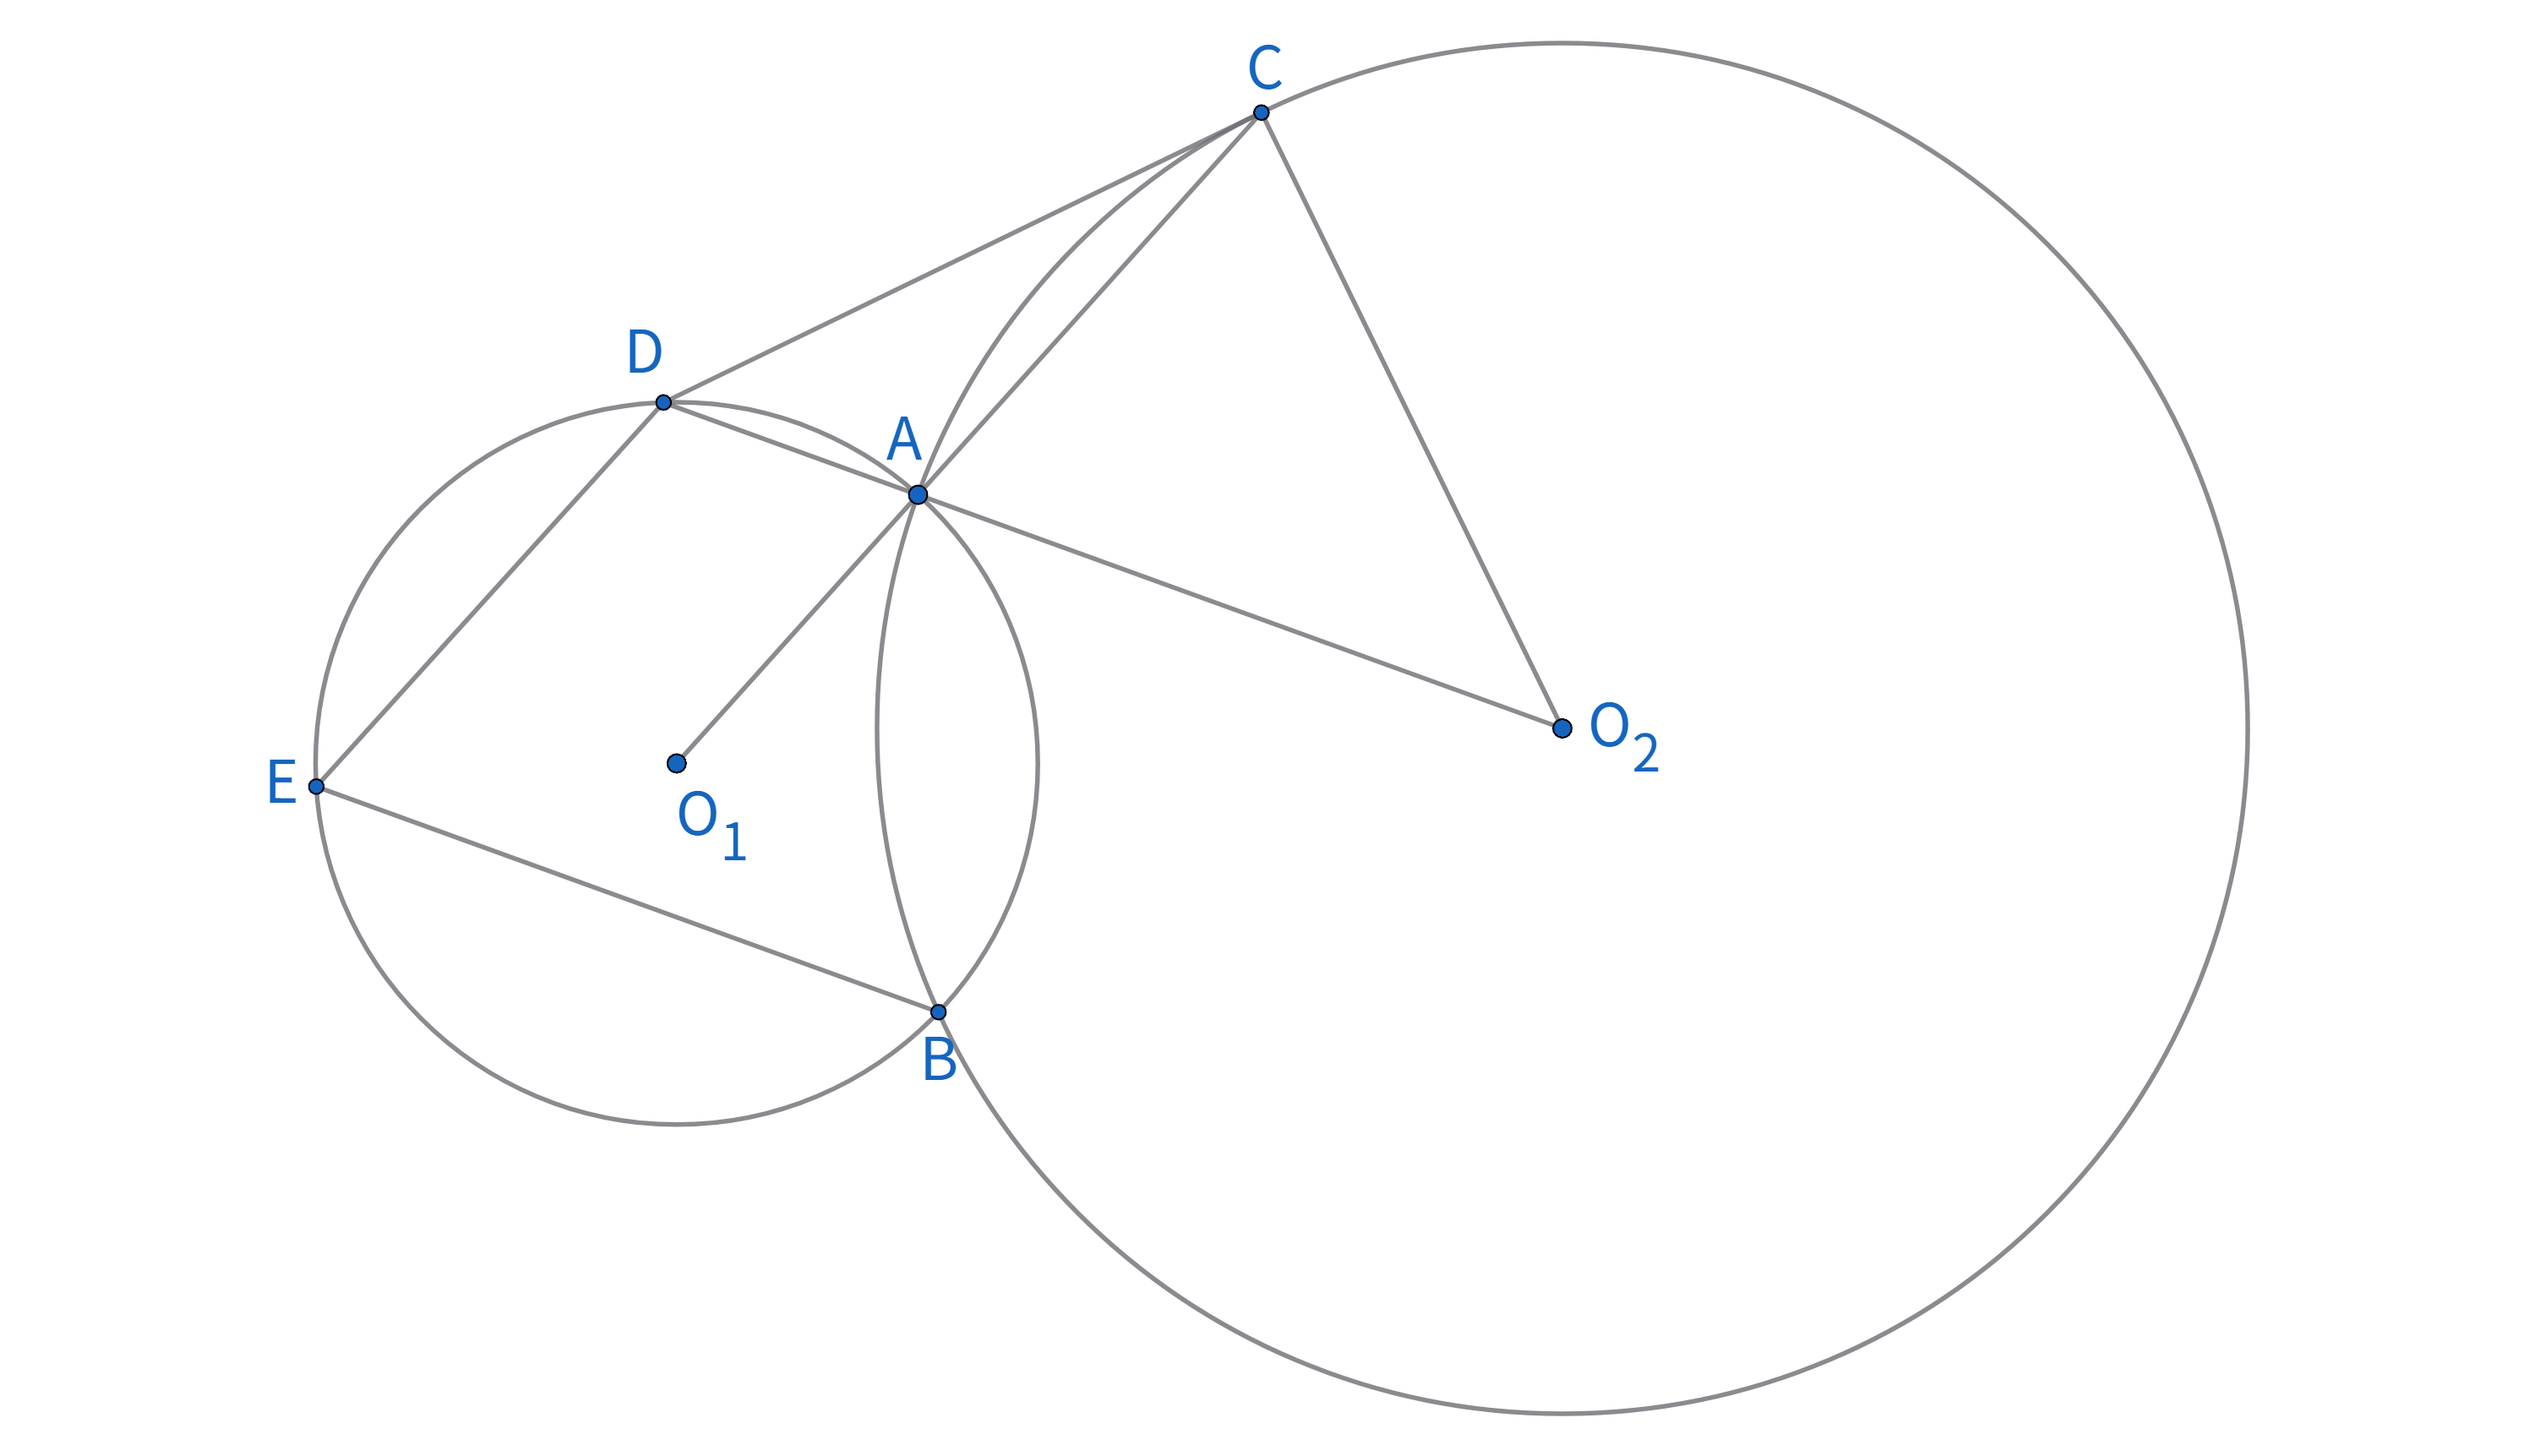
\includegraphics[width=0.6\linewidth]{figures/女子赛14年Q1.png}
\end{figure}


\subsection{Q6}
在锐角 $\triangle ABC$ 中,$AB > AC$,$D$、$E$ 分别是边 $AB$、$AC$ 的中点。$\triangle ADE$ 的外接圆与 $\triangle BCE$ 的外接圆交于点 $P$(异于点 $E$),$\triangle ADE$ 的外接圆与 $\triangle BCD$ 的外接圆交于点 $Q$(异于点 $D$)。求证:$AP = AQ$。
\begin{figure}[htbp]
    \centering
    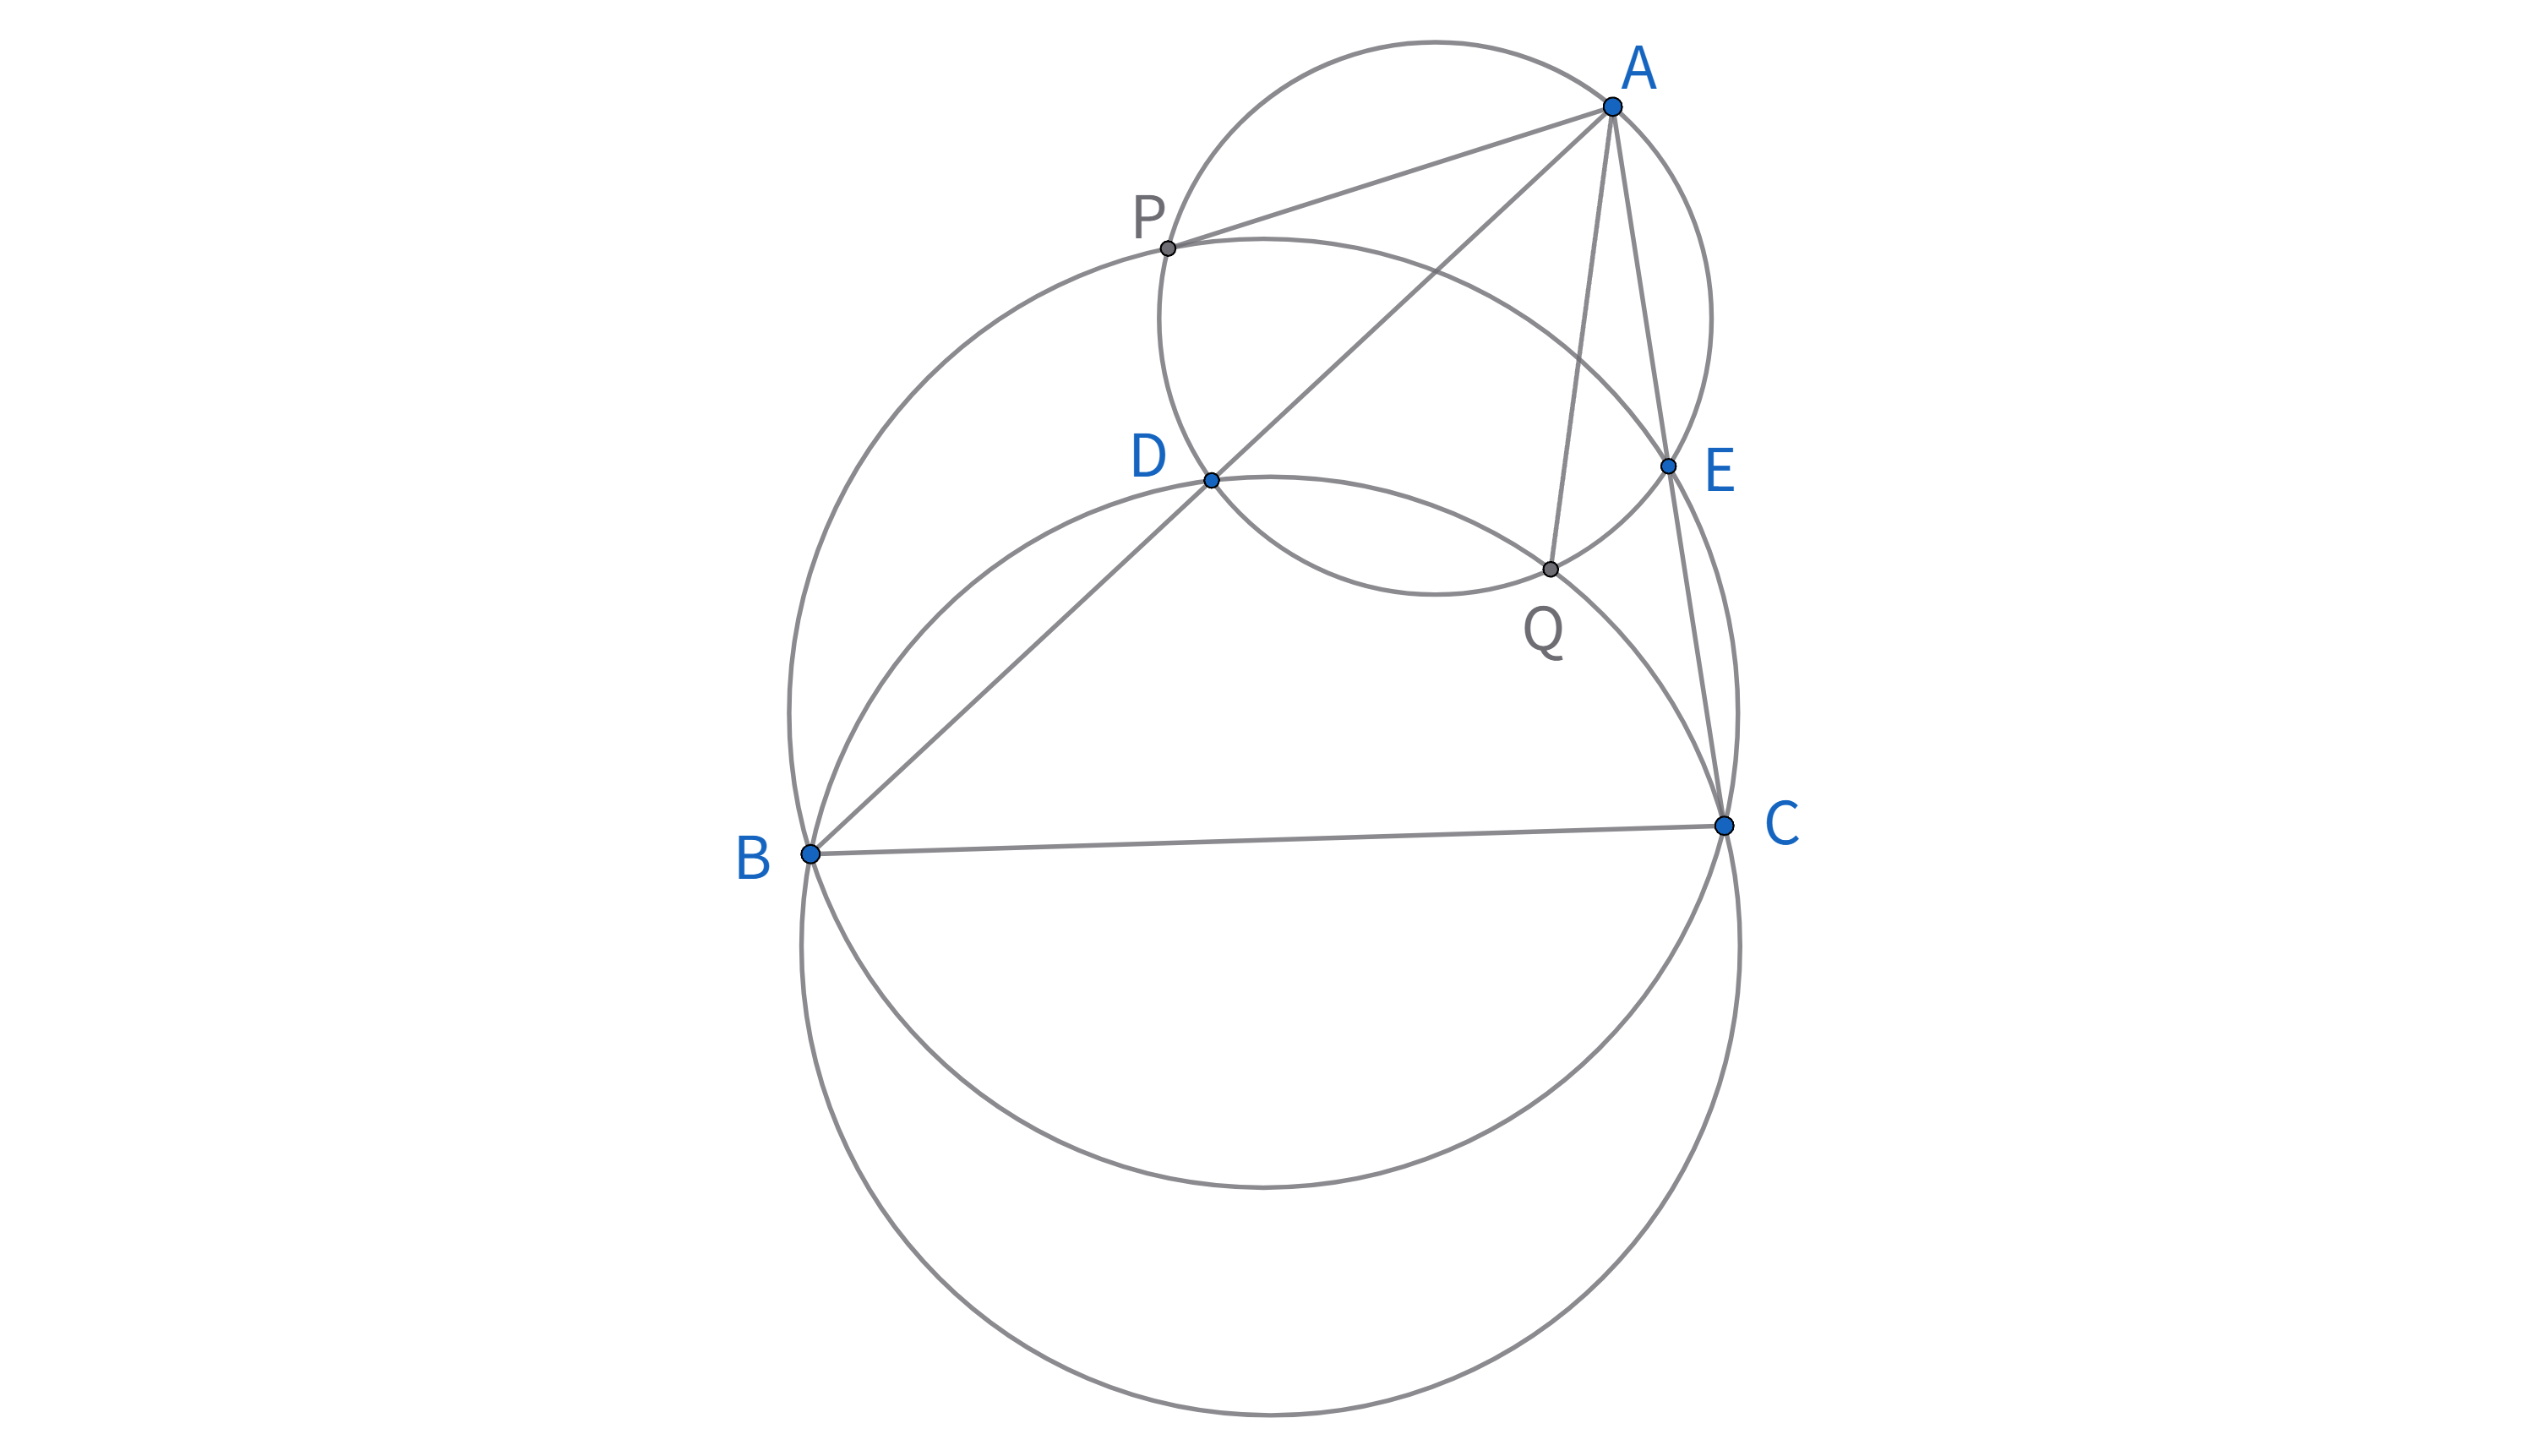
\includegraphics[width=0.7\linewidth]{figures/女子赛14年Q6.png}
\end{figure}


%-------------------------------------------------------------
\newpage 
\section{2013年}
\subsection{Q2}
在梯形 $ABCD$ 中,$AB \parallel CD$,$\odot O_1$ 与 $DA$、$AB$、$BC$ 三边相切,$\odot O_2$ 与 $BC$、$CD$、$DA$ 三边相切。设 $P$ 是 $\odot O_1$ 与边 $AB$ 的切点,$Q$ 是 $\odot O_2$ 与边 $CD$ 的切点。证明:$AC$、$BD$、$PQ$ 三线共点。
\begin{figure}[htbp]
    \centering
    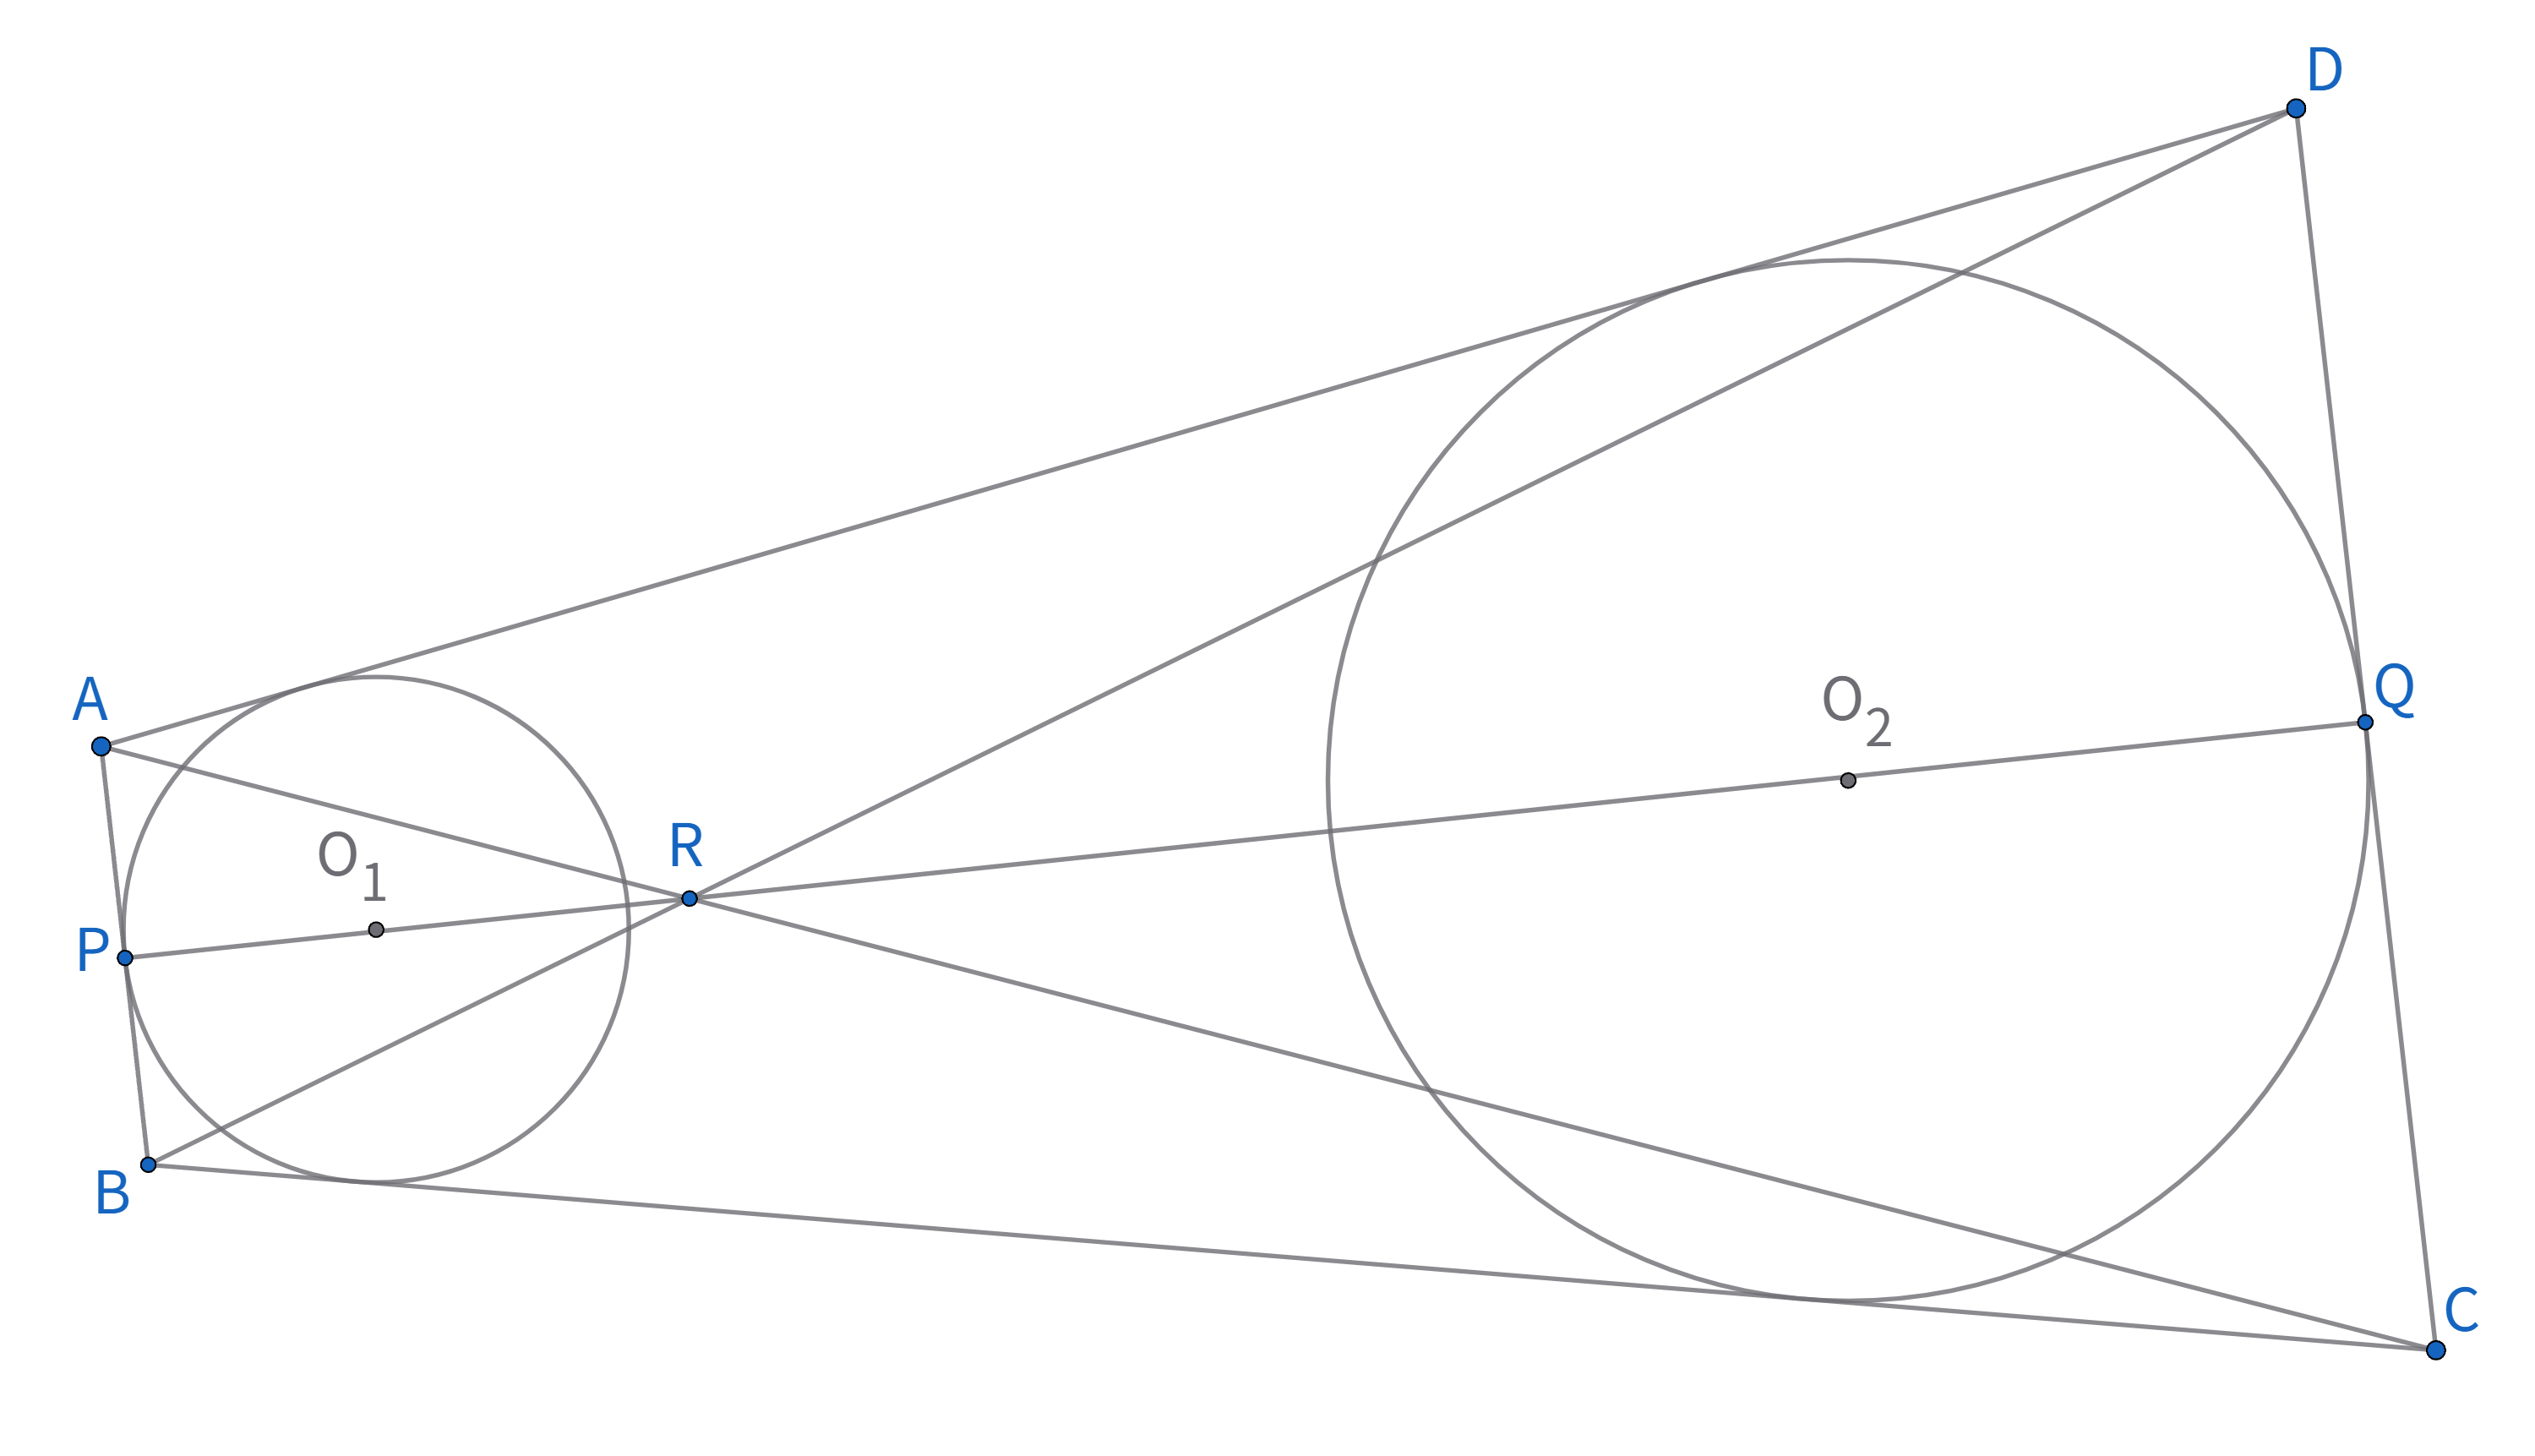
\includegraphics[width=0.7\linewidth]{figures/女子赛13年Q2.png}
\end{figure}


\subsection{Q7}
$\odot O_1$ 与 $\odot O_2$ 外切于点 $T$,四边形 $ABCD$ 内接于 $\odot O_1$,直线 $DA$、$CB$ 分别切 $\odot O_2$ 于点 $E$、$F$。直线 $BN$ 平分 $\angle ABF$ 并与线段 $EF$ 交于点 $N$。直线 $FT$ 交 $\widehat{AT}$(不包含点 $B$ 的弧)内于另一点 $M$。求证:点 $M$ 为 $\triangle BCN$ 的外心。
\begin{figure}[htbp]
    \centering
    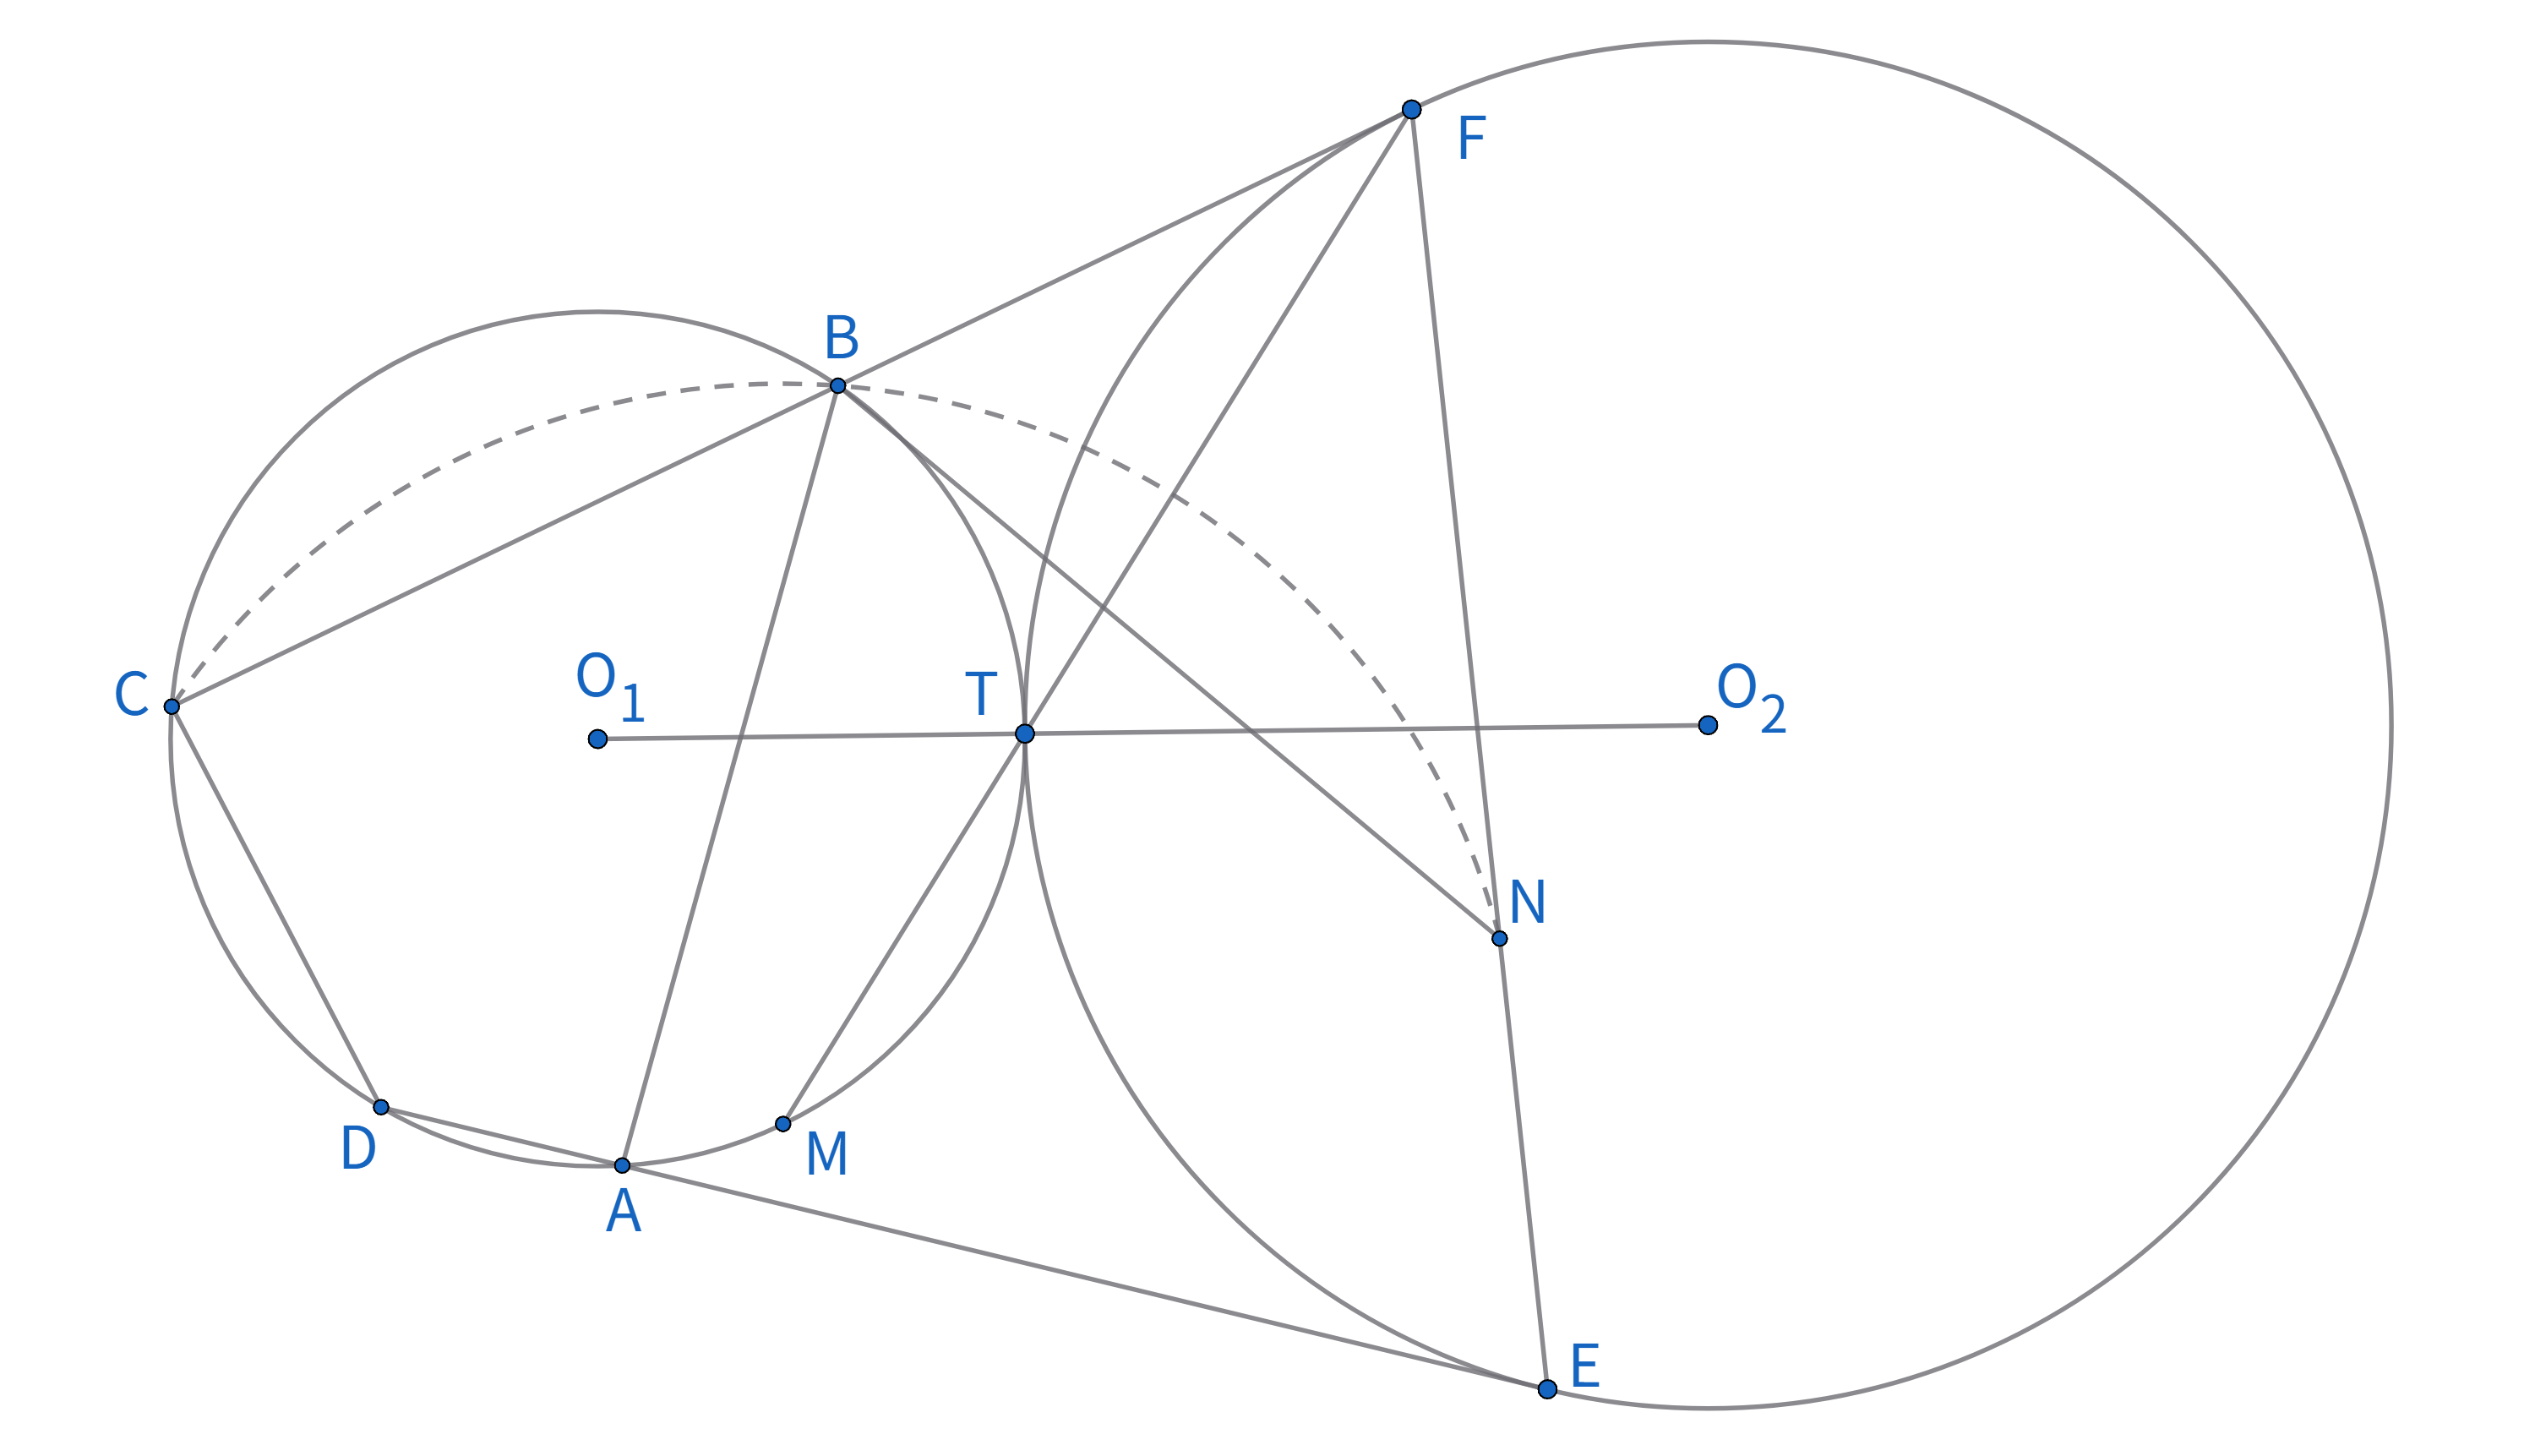
\includegraphics[width=0.7\linewidth]{figures/女子赛13年Q7.png}
\end{figure}


%-------------------------------------------------------------
\newpage 
\section{2012年}
\subsection{Q2}
圆 $\Gamma_1$、$\Gamma_2$ 外切于点 $T$,点 $A$、$E$ 在圆 $\Gamma_1$ 上,直线 $AB$、$DE$ 分别与圆 $\Gamma_2$ 相切于点 $B$、$D$,直线 $AE$ 与 $BD$ 相交于点 $P$。求证:
(1) $\frac{AB}{AT} = \frac{ED}{ET}$;
(2) $\angle ATP + \angle ETP = 180^\circ$。
\begin{figure}[htbp]
    \centering
    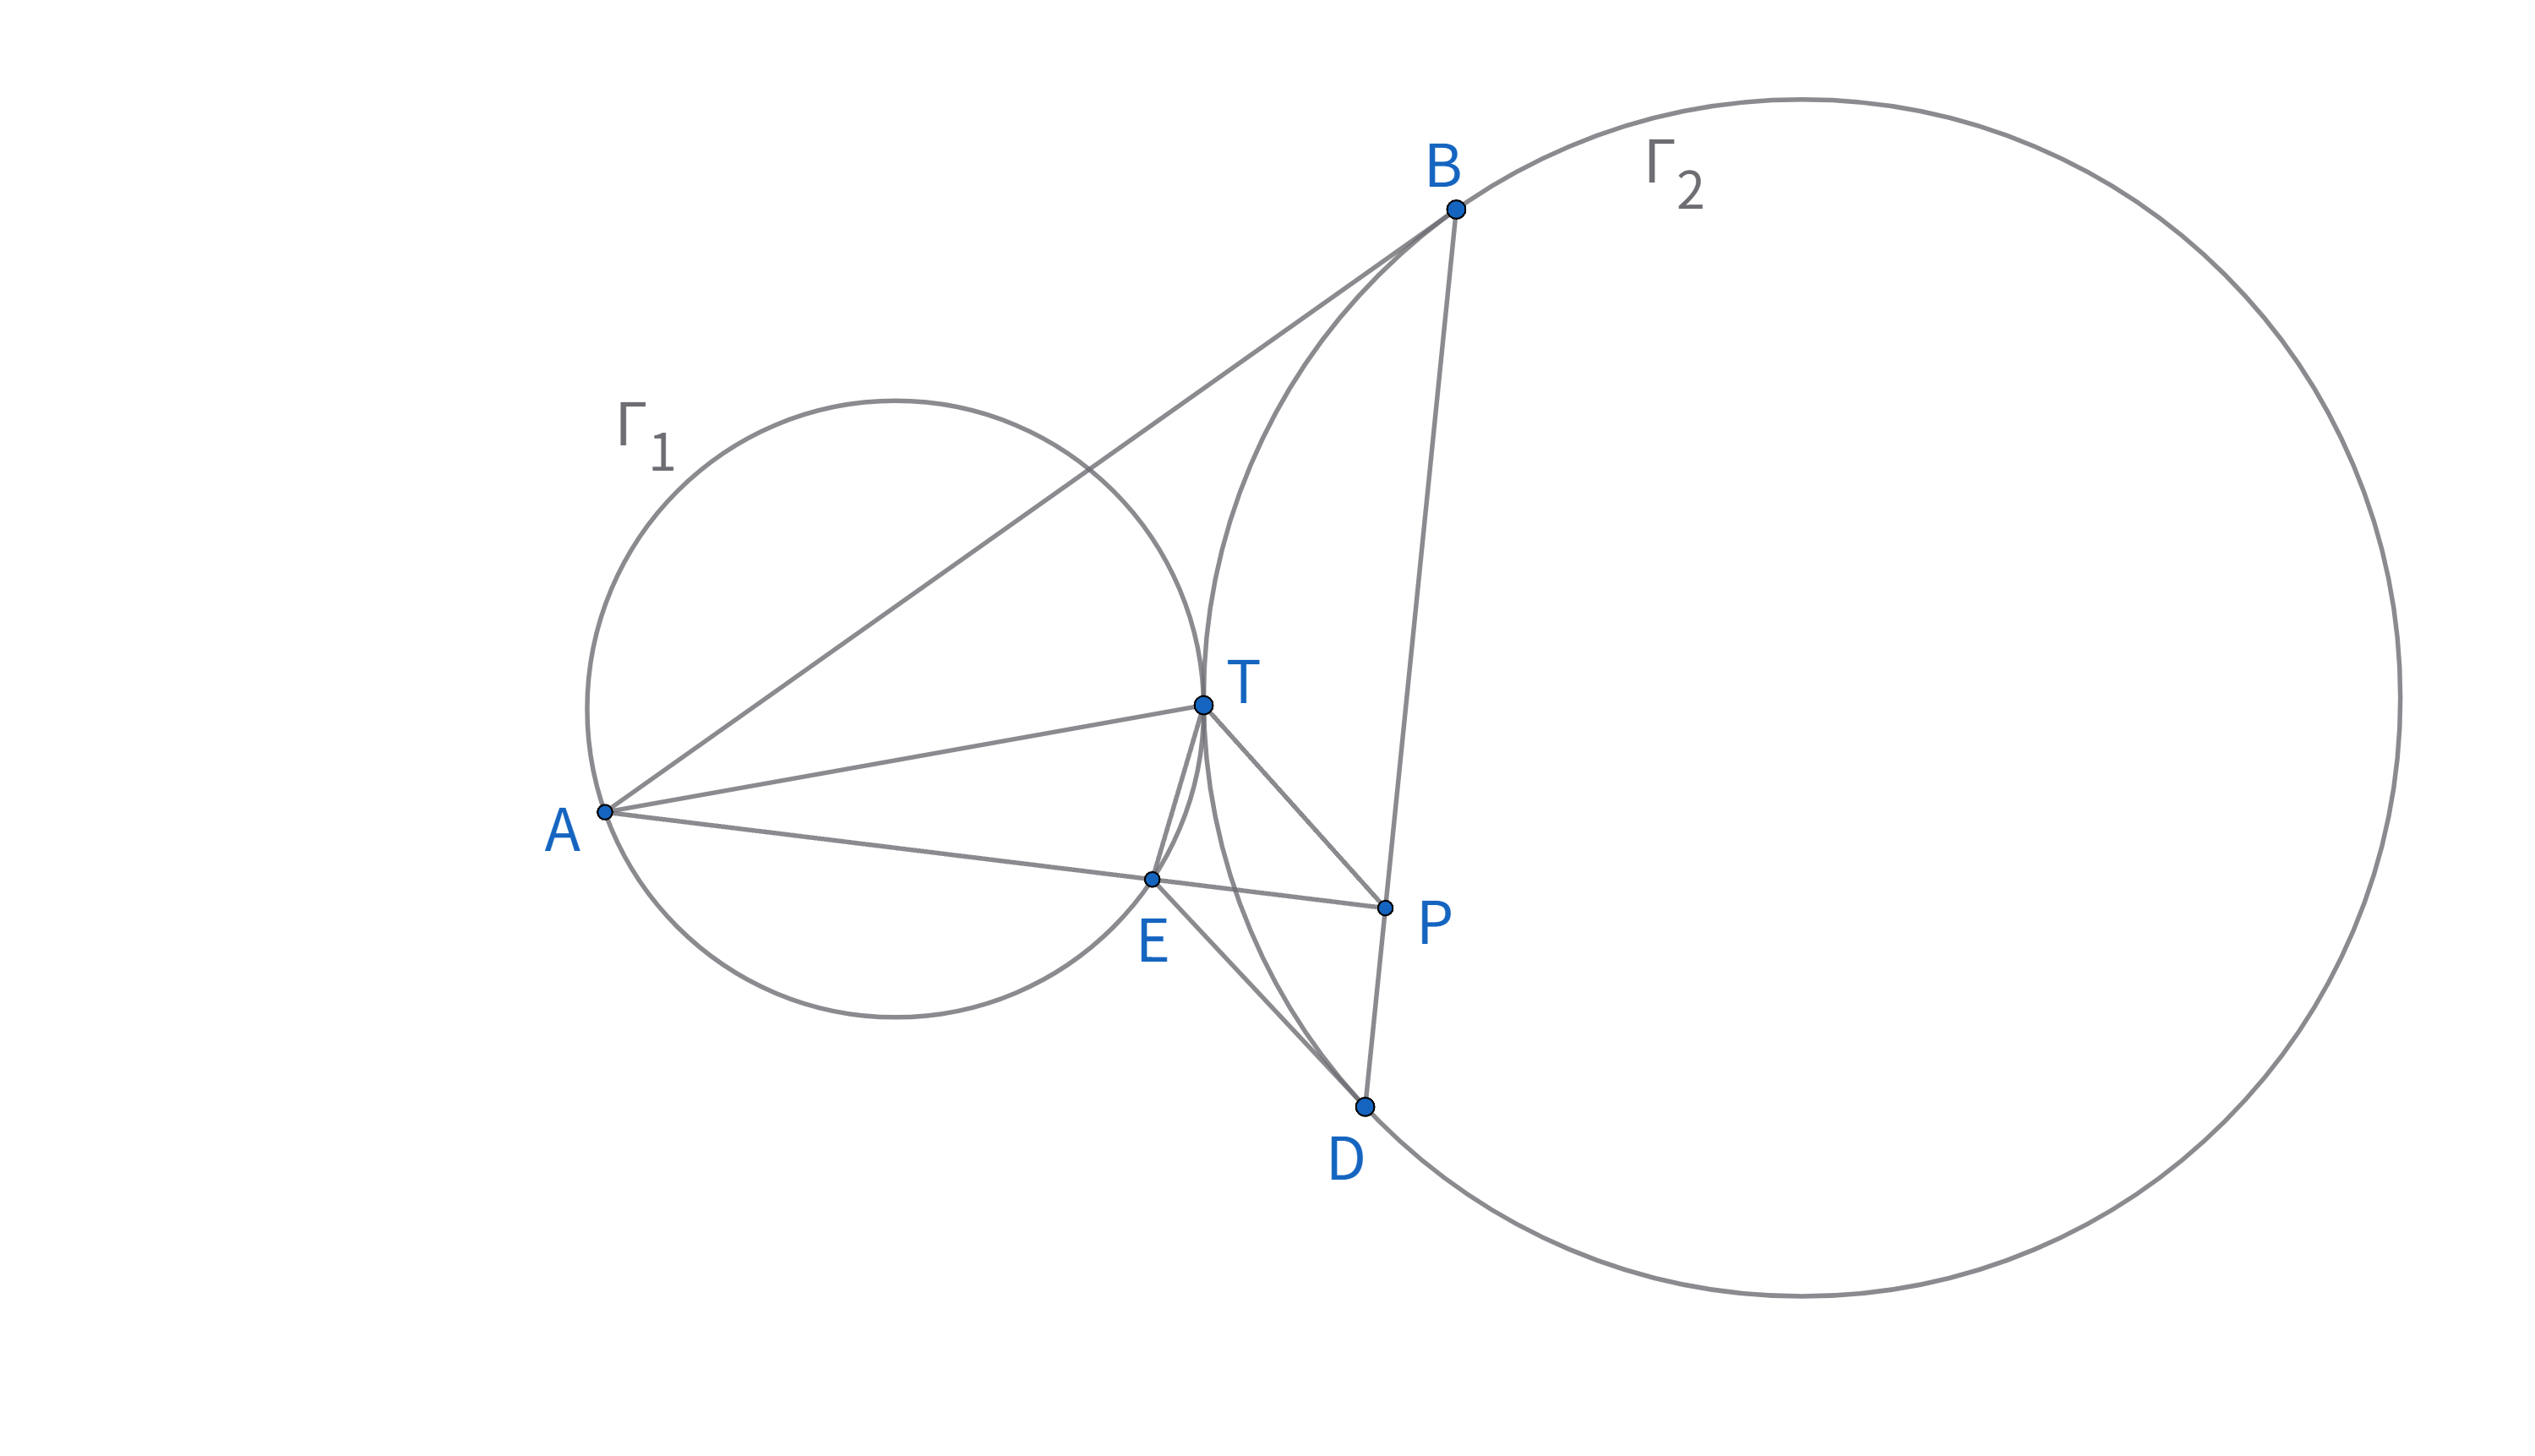
\includegraphics[width=0.8\linewidth]{figures/女子赛12年Q2.png}
\end{figure}


\subsection{Q5}
$\triangle ABC$ 的内切圆 $\odot I$ 与边 $AB$、$AC$ 分别相切于点 $D$、$E$,$\triangle BCI$ 的外心为 $O$。证明:$\angle ODB = \angle OEC$。
\begin{figure}[htbp]
    \centering
    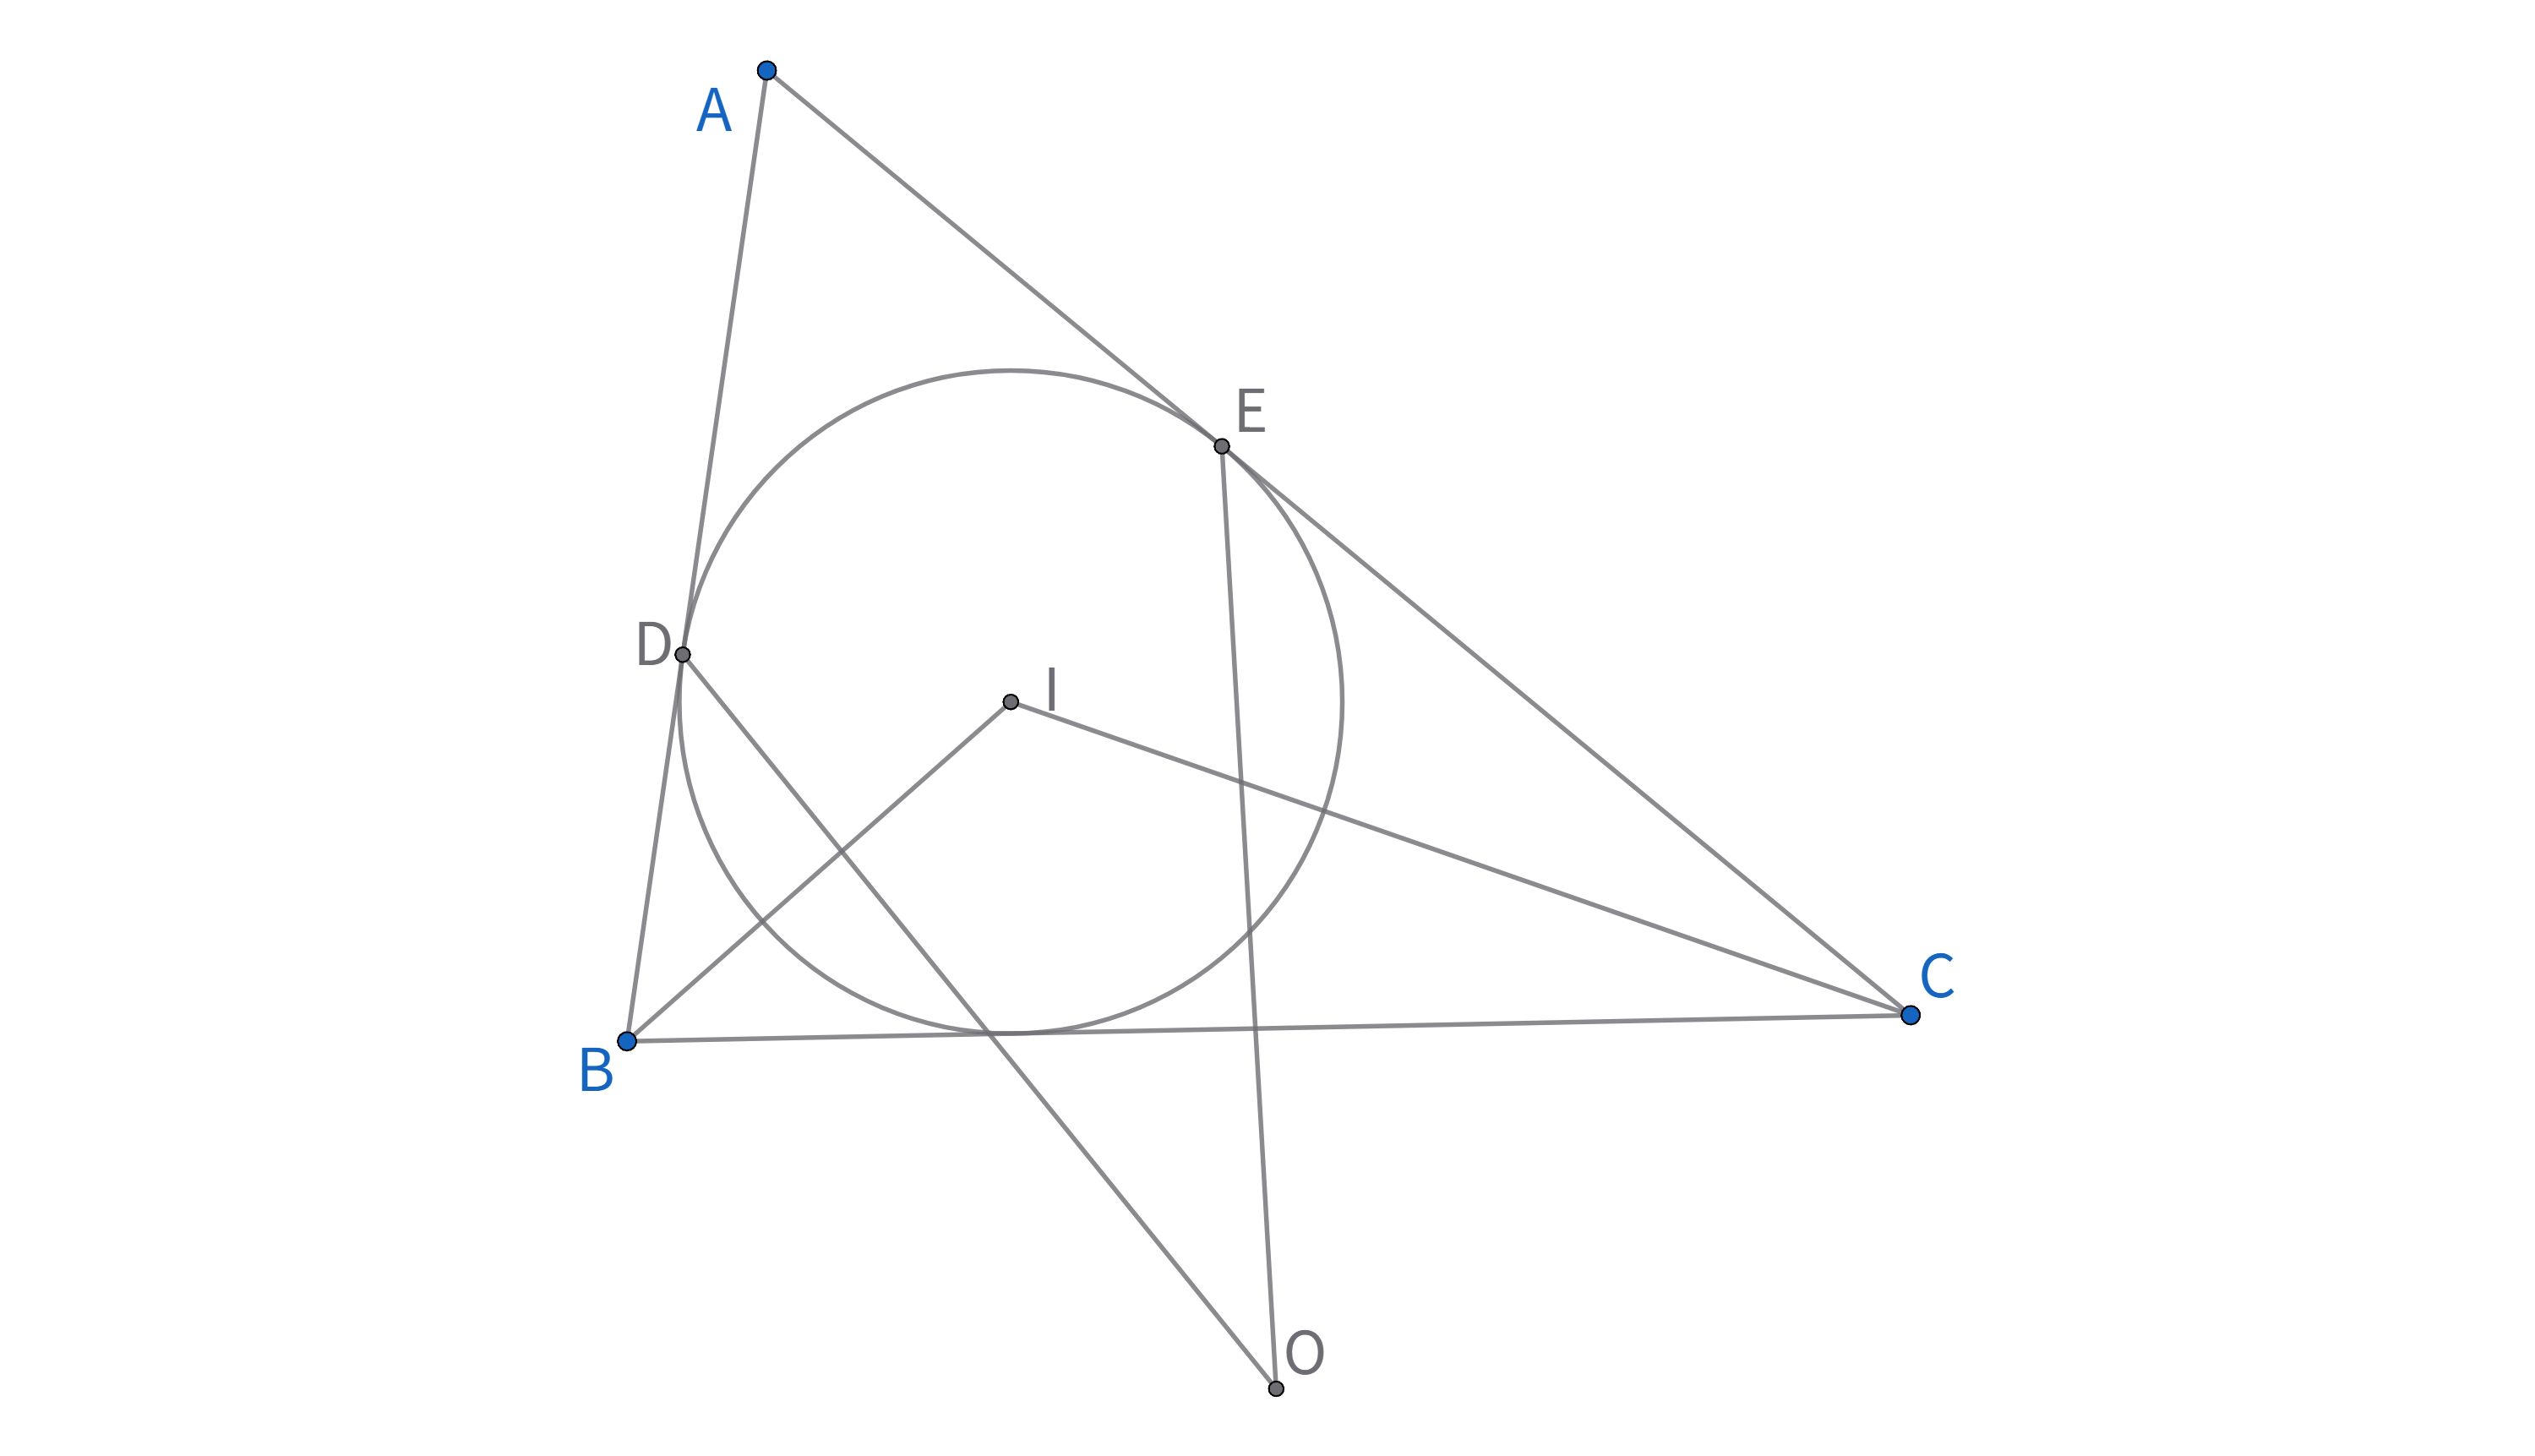
\includegraphics[width=0.8\linewidth]{figures/女子赛12年Q5.png}
\end{figure}



%-------------------------------------------------------------
\newpage 
\section{2011年}
\subsection{Q2}
四边形 $ABCD$ 的对角线 $AC$ 与 $BD$ 相交于点 $E$,边 $AB$、$CD$ 的中垂线相交于点 $F$,点 $M$、$N$ 分别为边 $AB$、$CD$ 的中点,直线 $EF$ 分别与边 $BC$、$AD$ 相交于点 $P$、$Q$。若 $MF \cdot CD = NF \cdot AB$ 且 $DQ \cdot BP = AQ \cdot CP$,求证:$PQ \perp BC$。
\begin{figure}[htbp]
    \centering
    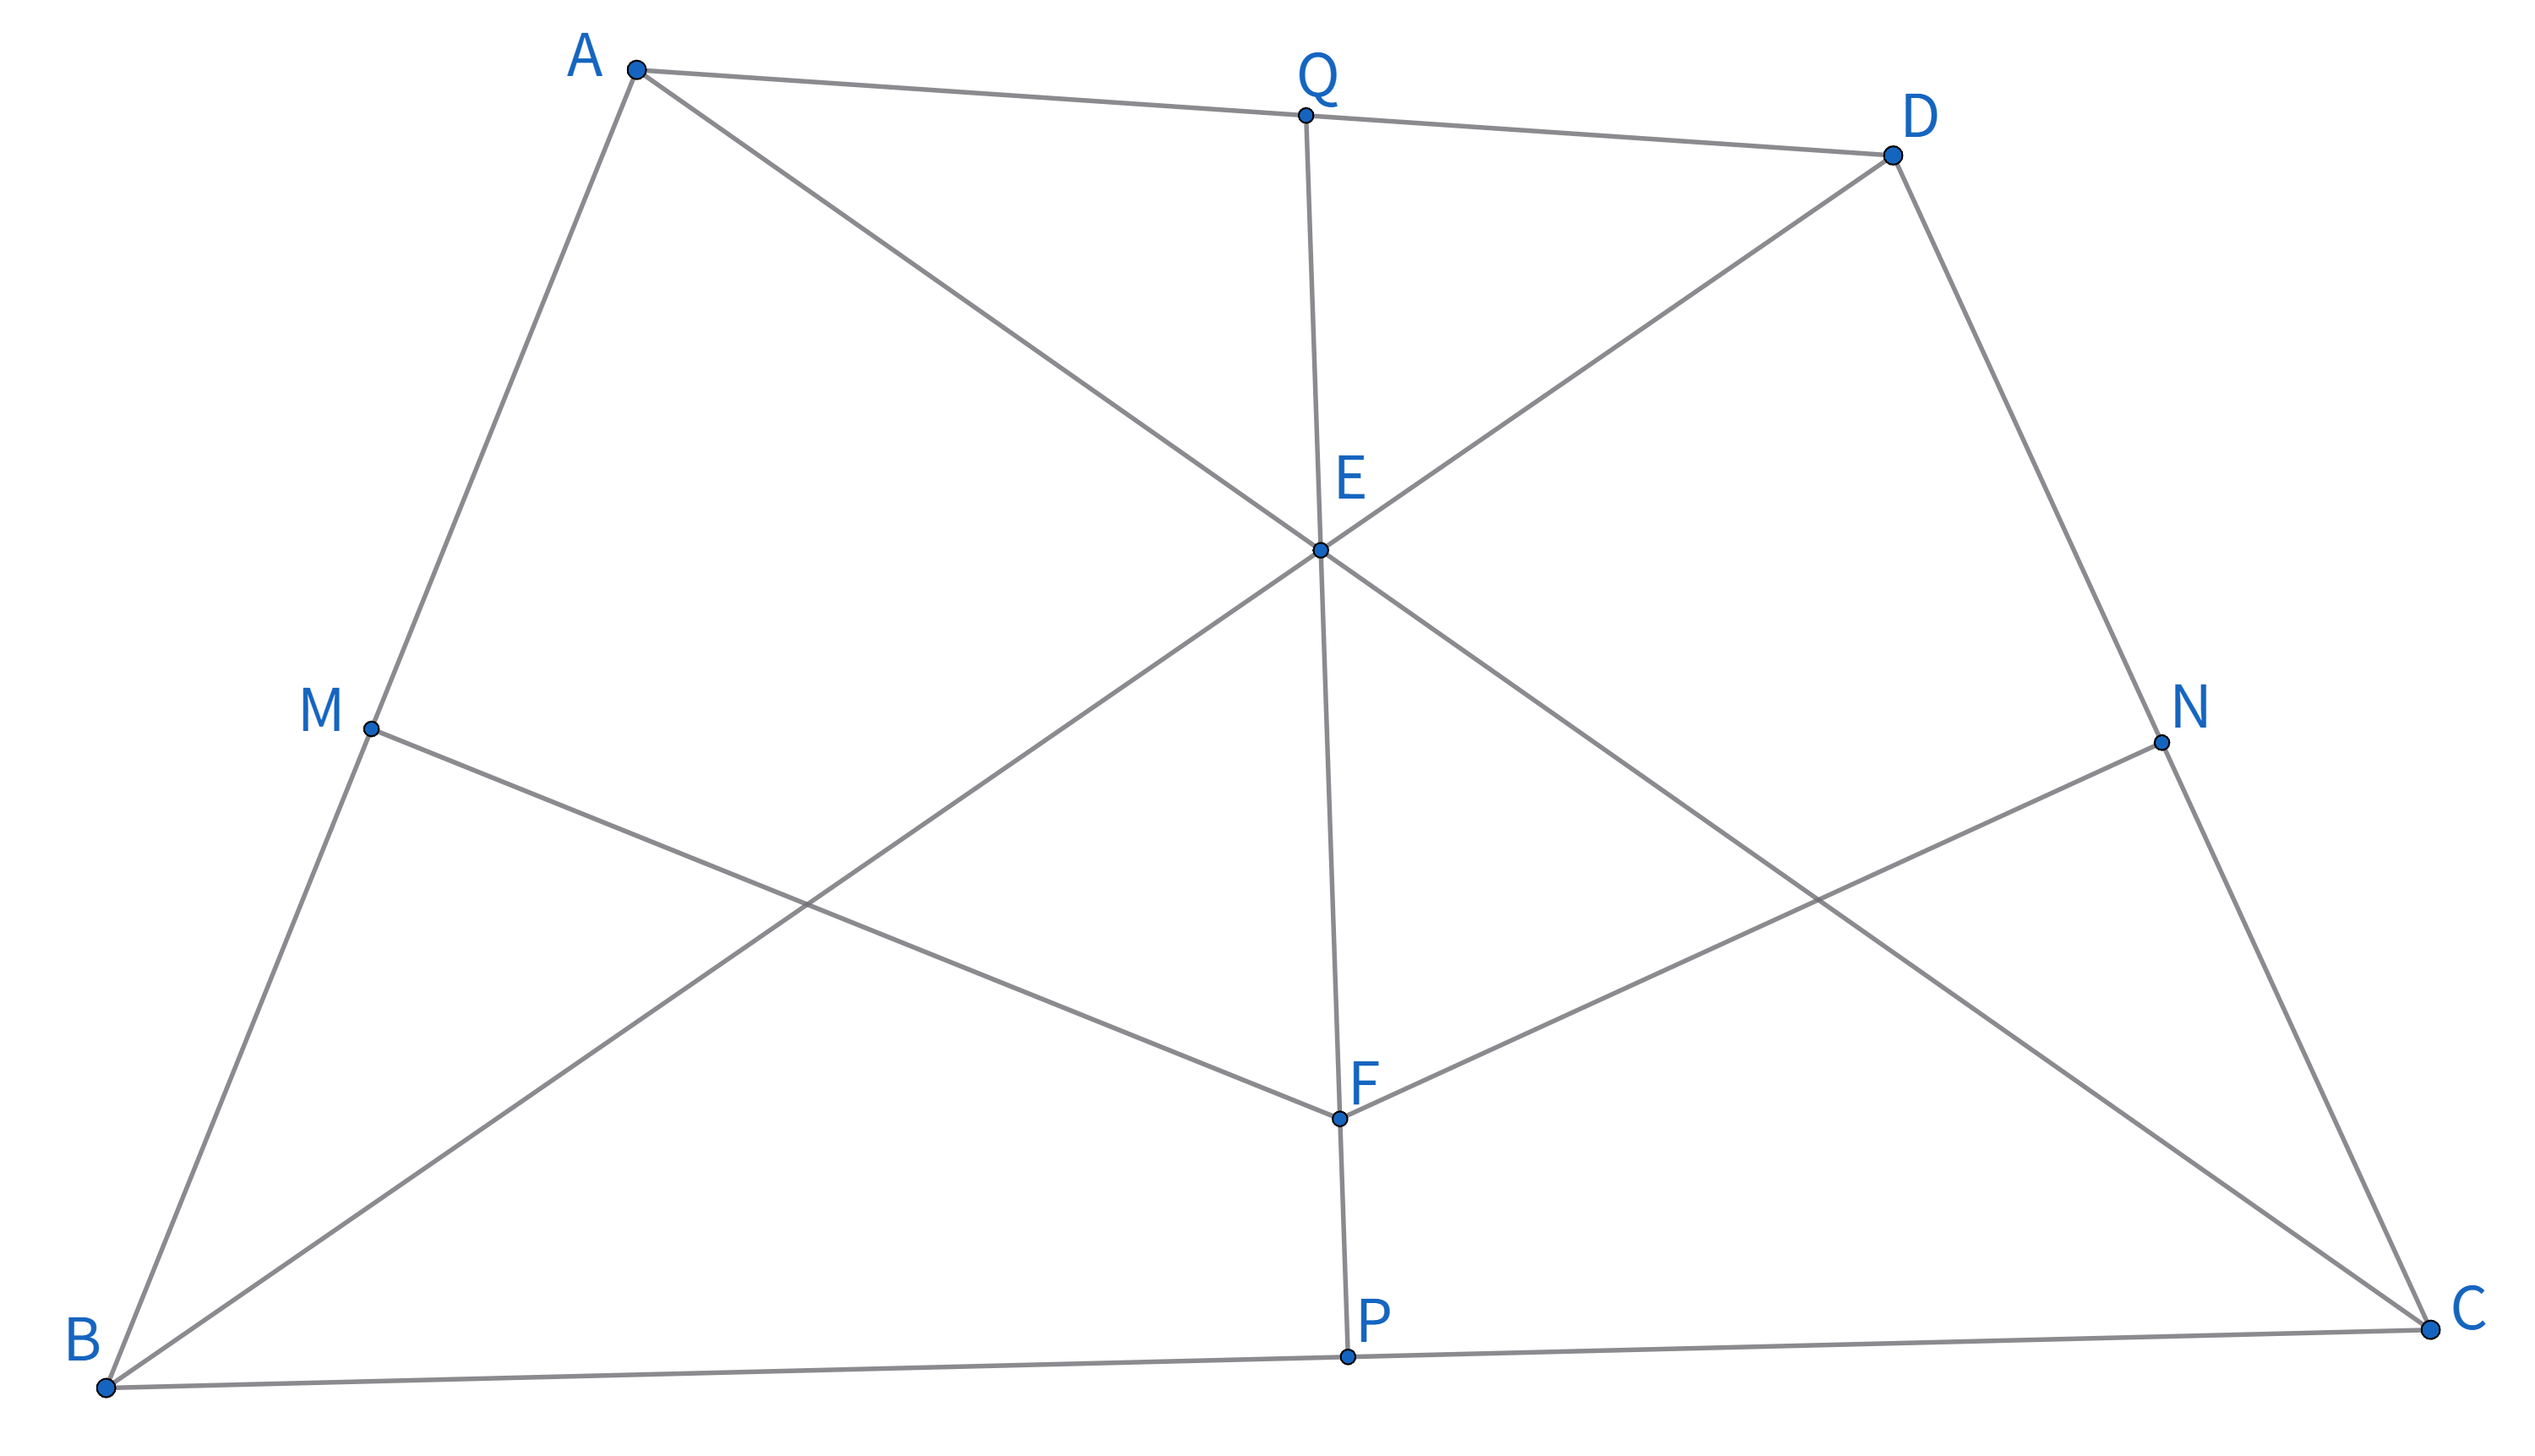
\includegraphics[width=0.7\linewidth]{figures/女子赛11年Q2.png}
\end{figure}

\subsection{Q8}
$\odot O$ 为 $\triangle ABC$ 中 $BC$ 边上的旁切圆,点 $D$、$E$ 分别在线段 $AB$、$AC$ 上,使得 $DE \parallel BC$。$\odot O_1$ 为 $\triangle ADE$ 的内切圆,$O_1B$ 交 $DO$ 于点 $F$,$O_1C$ 交 $EO$ 于点 $G$。$\odot O$ 切 $BC$ 于点 $M$,$\odot O_1$ 切 $DE$ 于点 $N$。求证:$MN$ 平分线段 $FG$。
\begin{figure}[htbp]
    \centering
    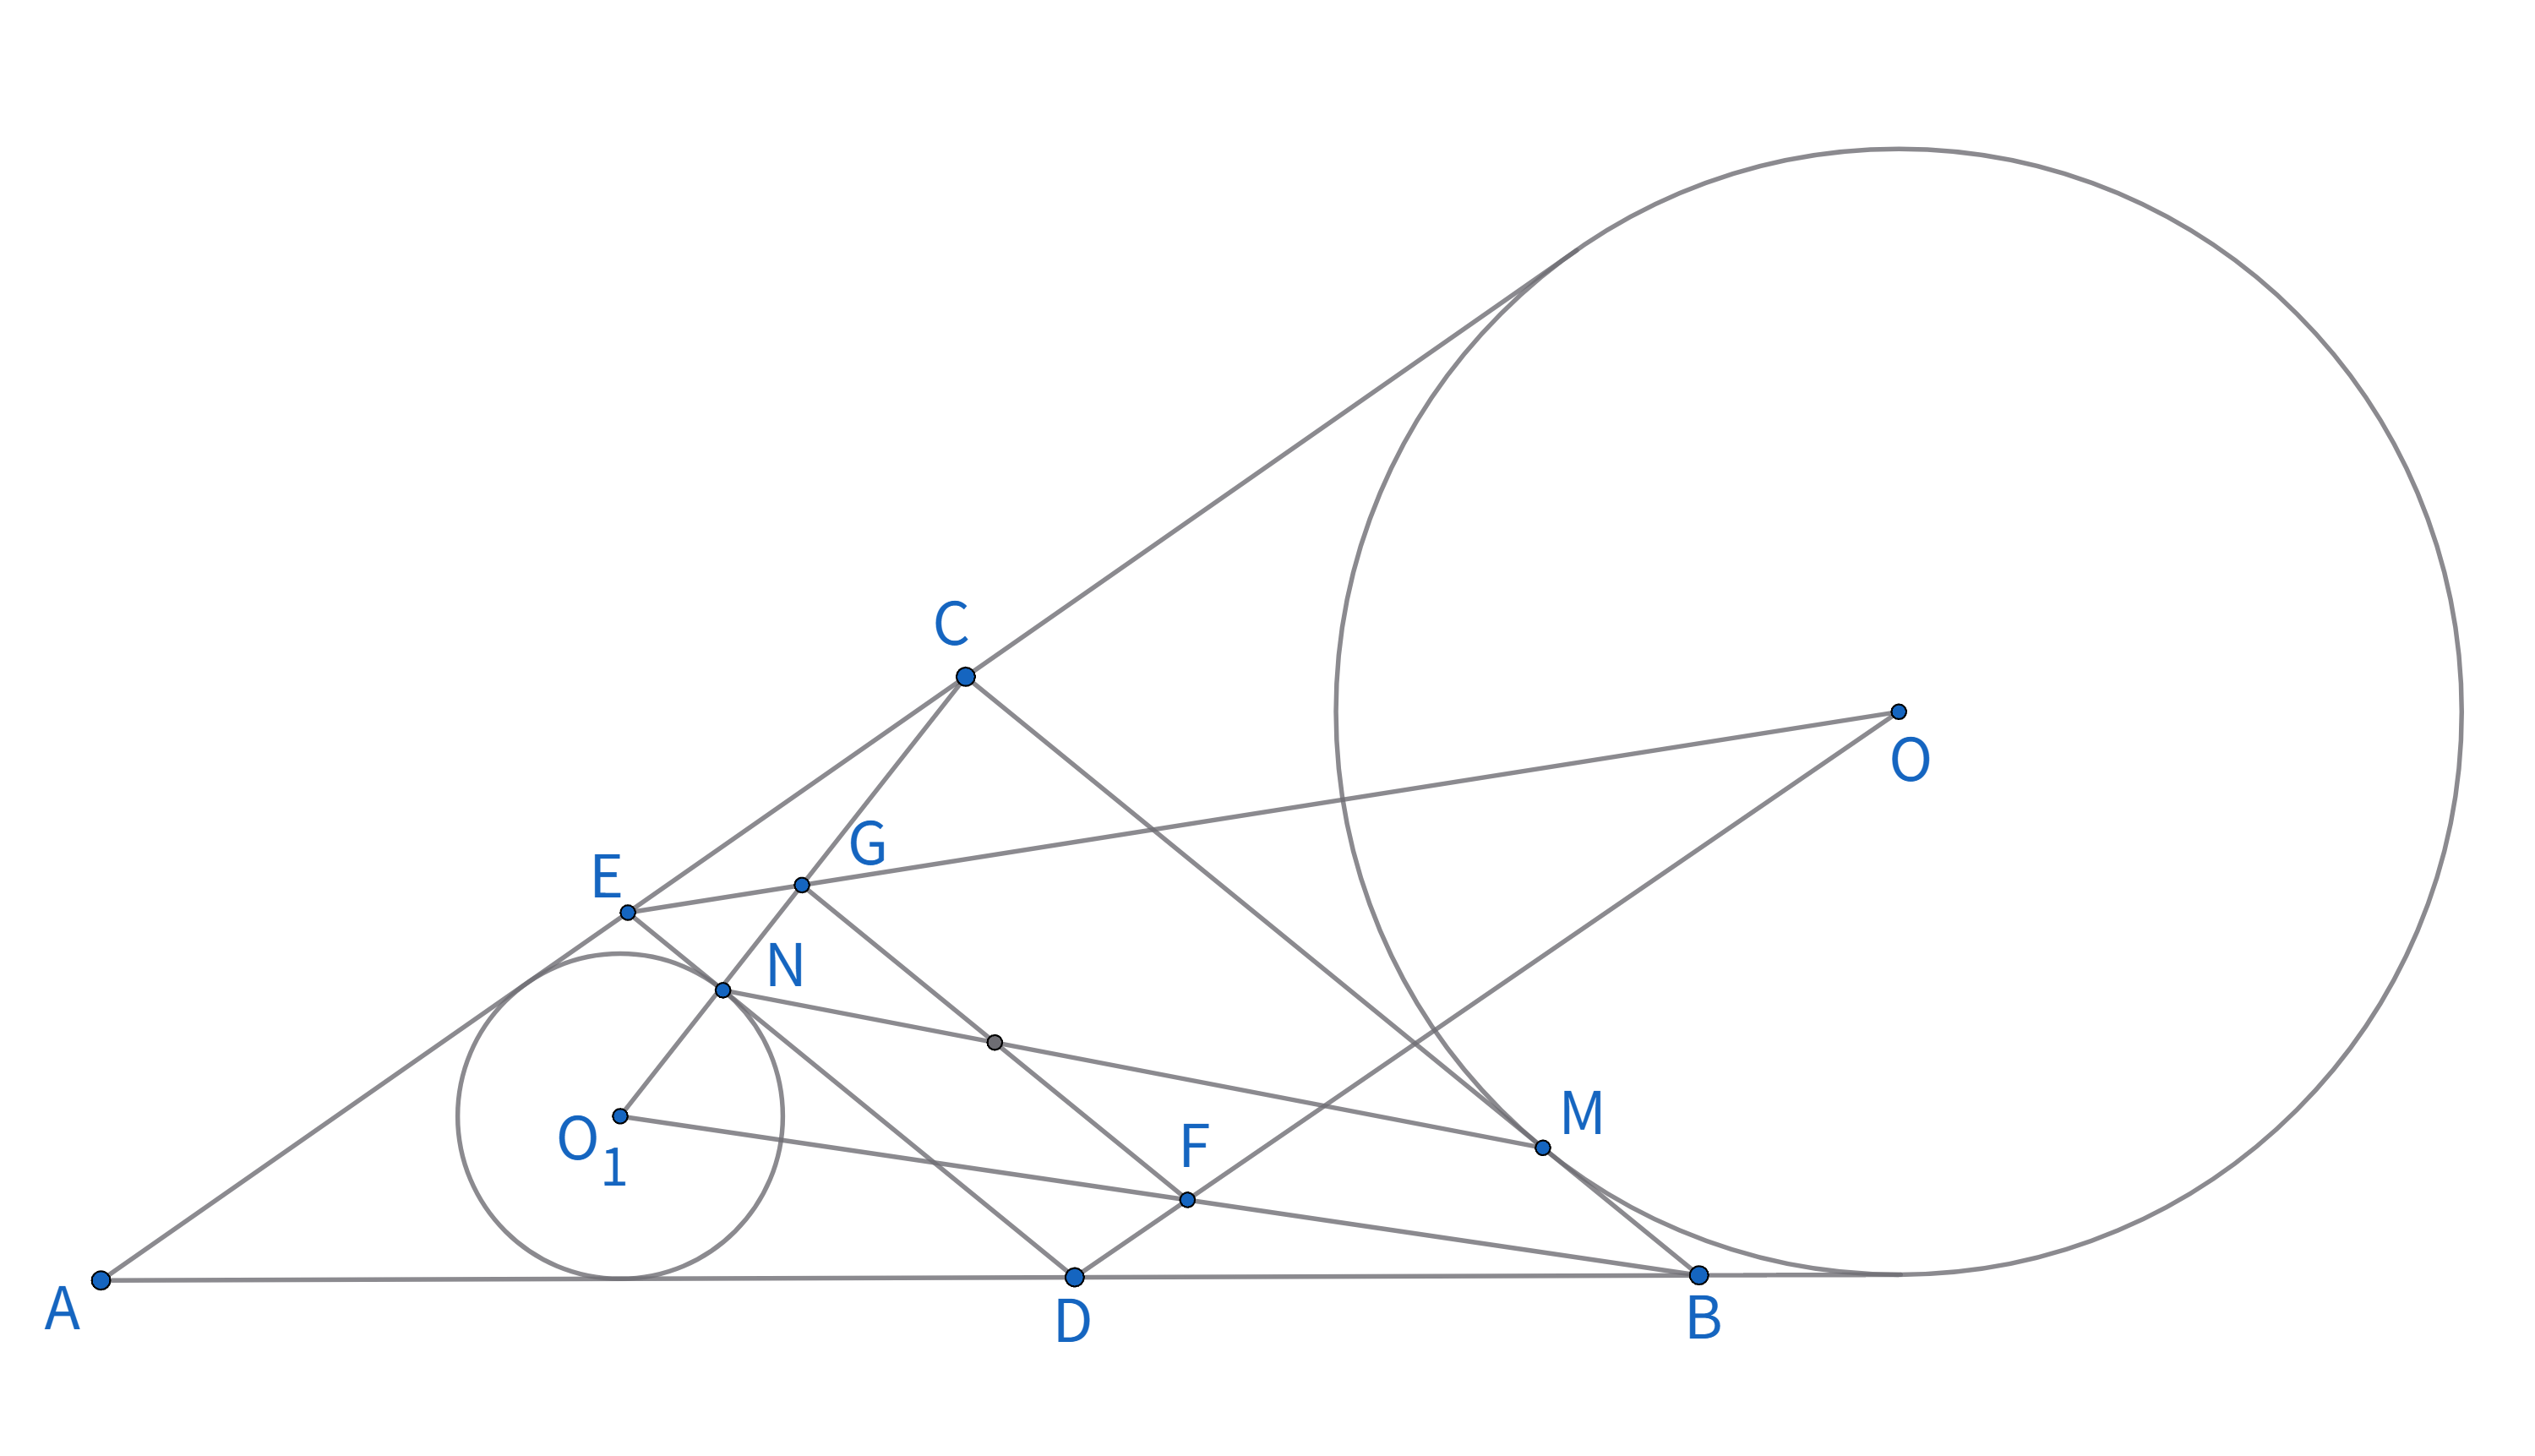
\includegraphics[width=0.7\linewidth]{figures/女子赛11年Q8.png}
\end{figure}


%-------------------------------------------------------------
\newpage
\section{2010年}
\subsection{Q2}
在 $\triangle ABC$ 中,$AB = AC$,$D$ 为边 $BC$ 的中点。$E$ 是 $\triangle ABC$ 外一点,满足 $CE \perp AB$,$BE = BD$。过线段 $BE$ 的中点 $M$ 作直线 $MF \perp BE$,交 $\triangle ABD$ 的外接圆的劣弧 $\overset{\frown}{AD}$ 于点 $F$。求证:$ED \perp DF$。
\begin{figure}[htbp]
    \centering
    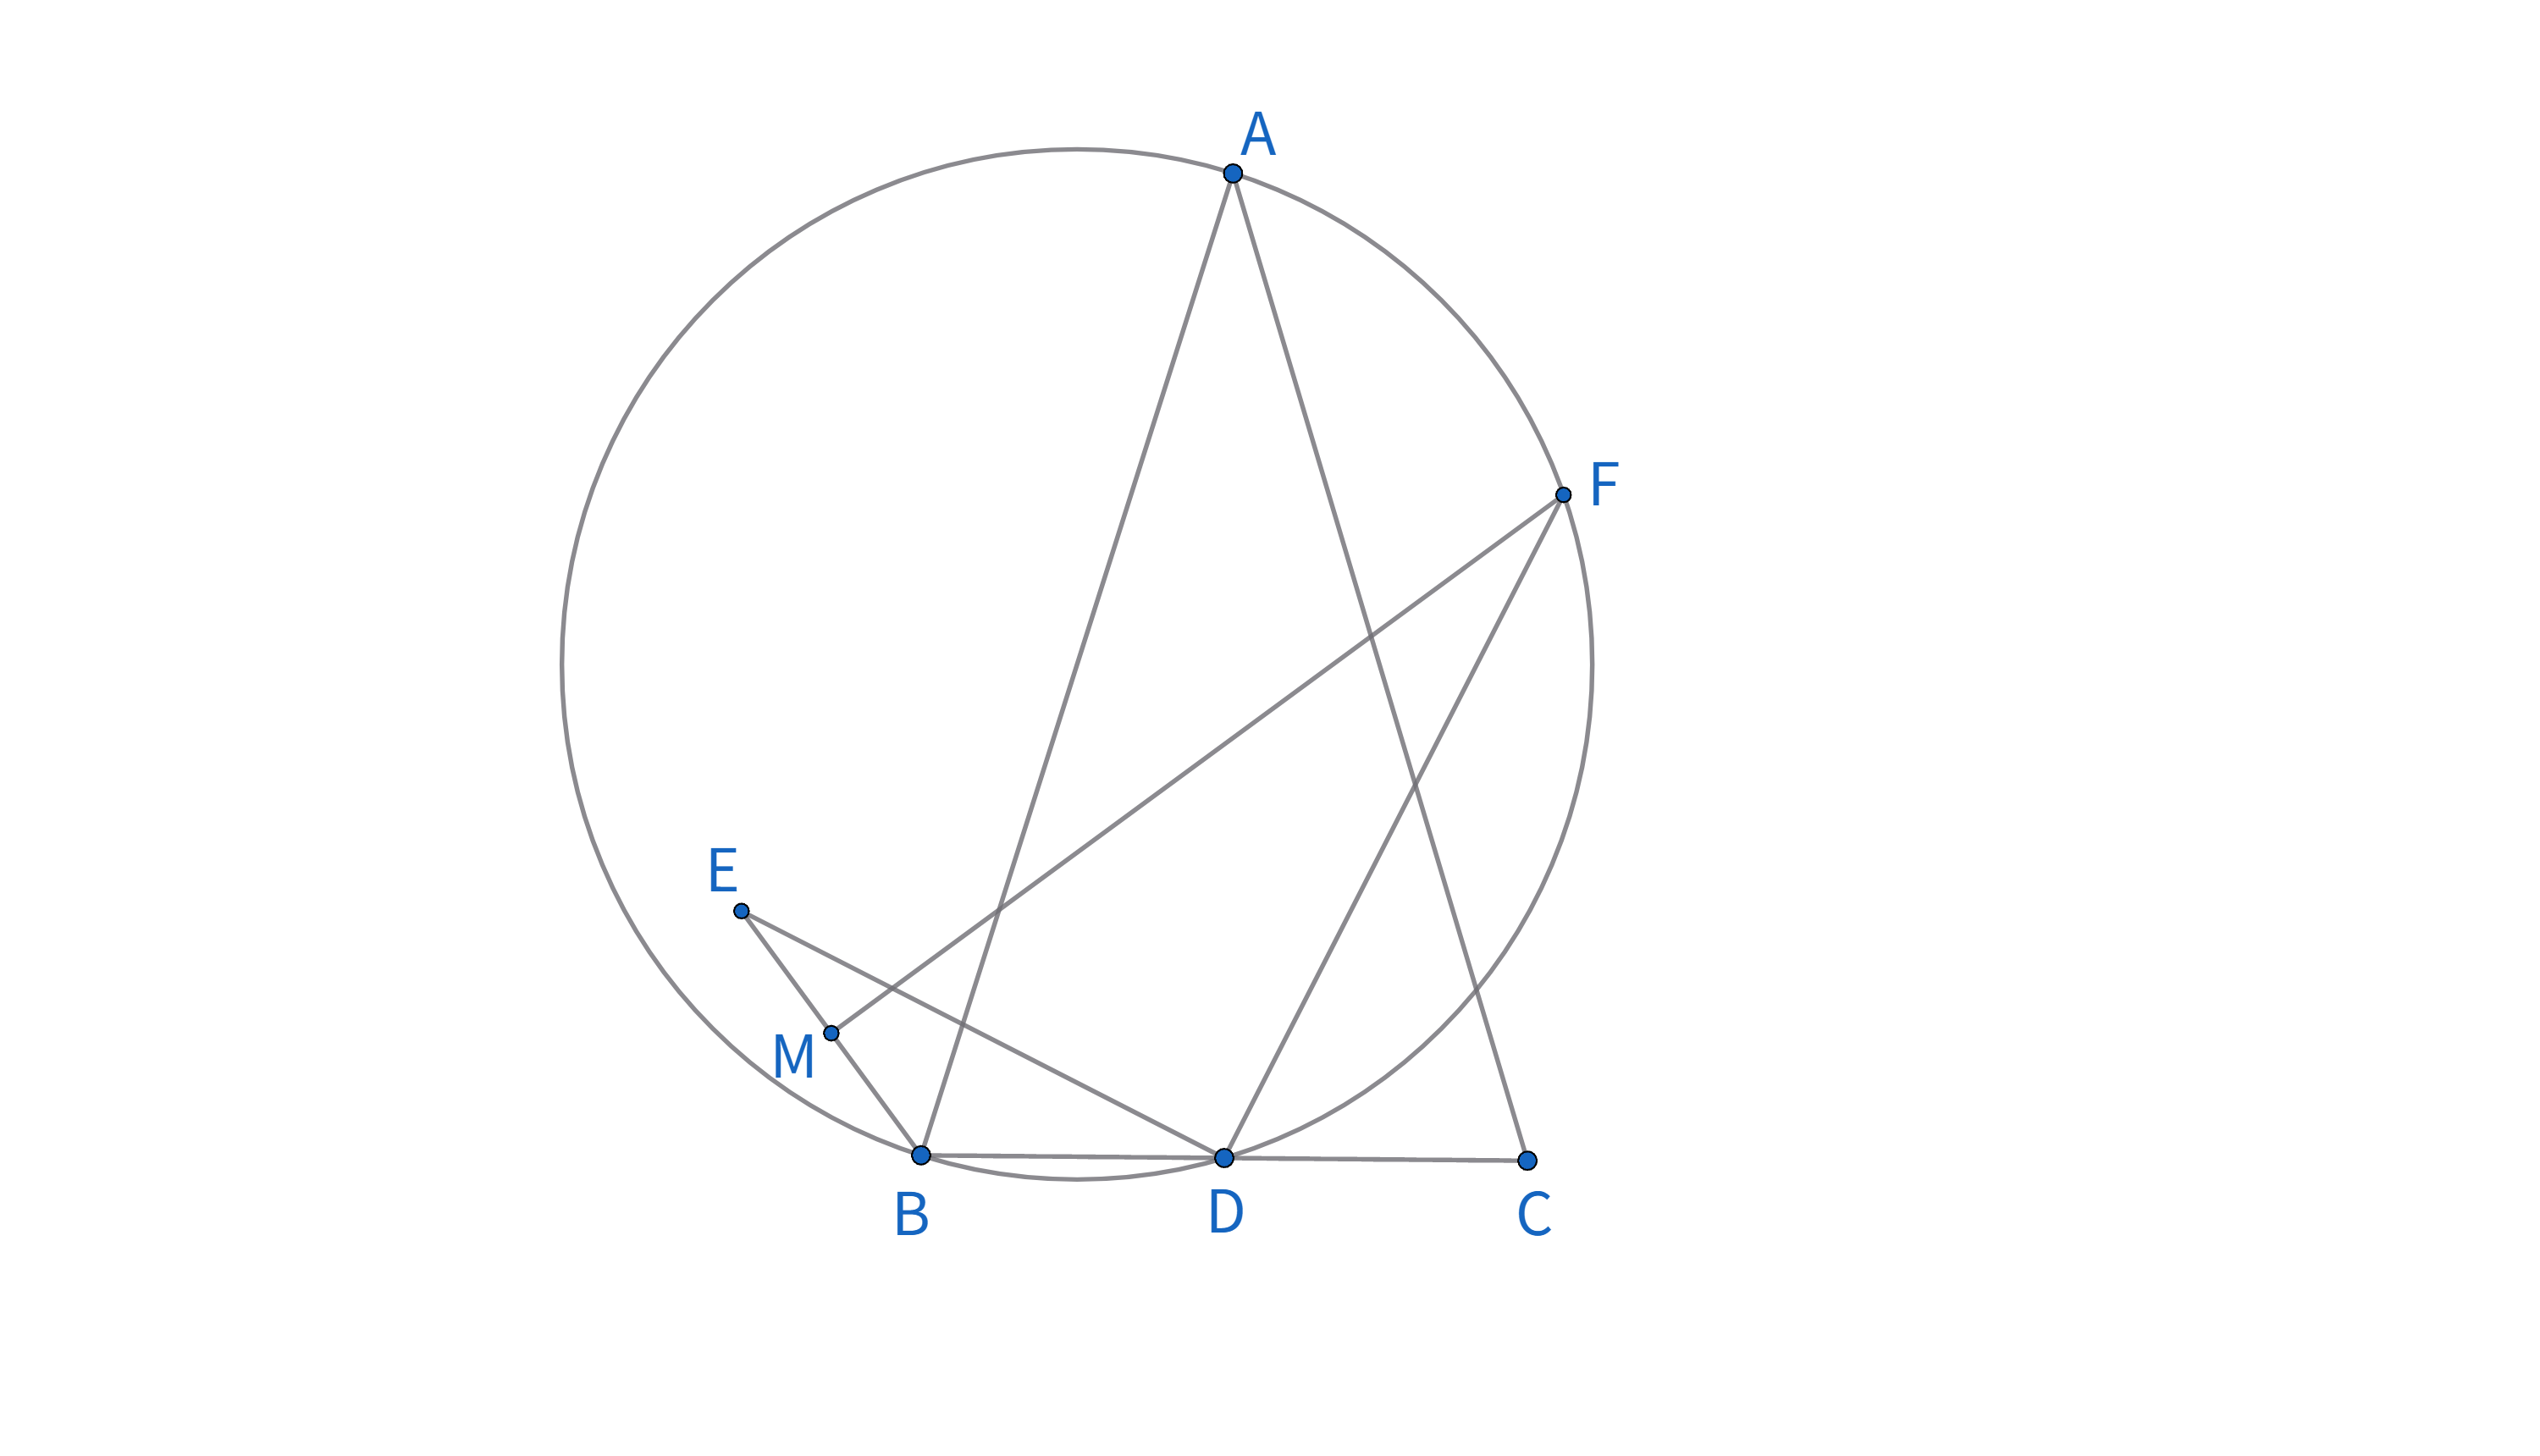
\includegraphics[width=0.8\linewidth]{figures/女子赛10年Q2.png}
\end{figure}

\subsection{Q6}
在锐角 $\triangle ABC$ 中,$AB > AC$,$M$ 为 $BC$ 的中点,$\angle BAC$ 的外角平分线交直线 $BC$ 于点 $P$。点 $K$、$F$ 在直线 $PA$ 上,使得 $MF \perp BC$,$MK \perp PA$。求证:$BC^2 = 4PF \cdot AK$。
\begin{figure}[htbp]
    \centering
    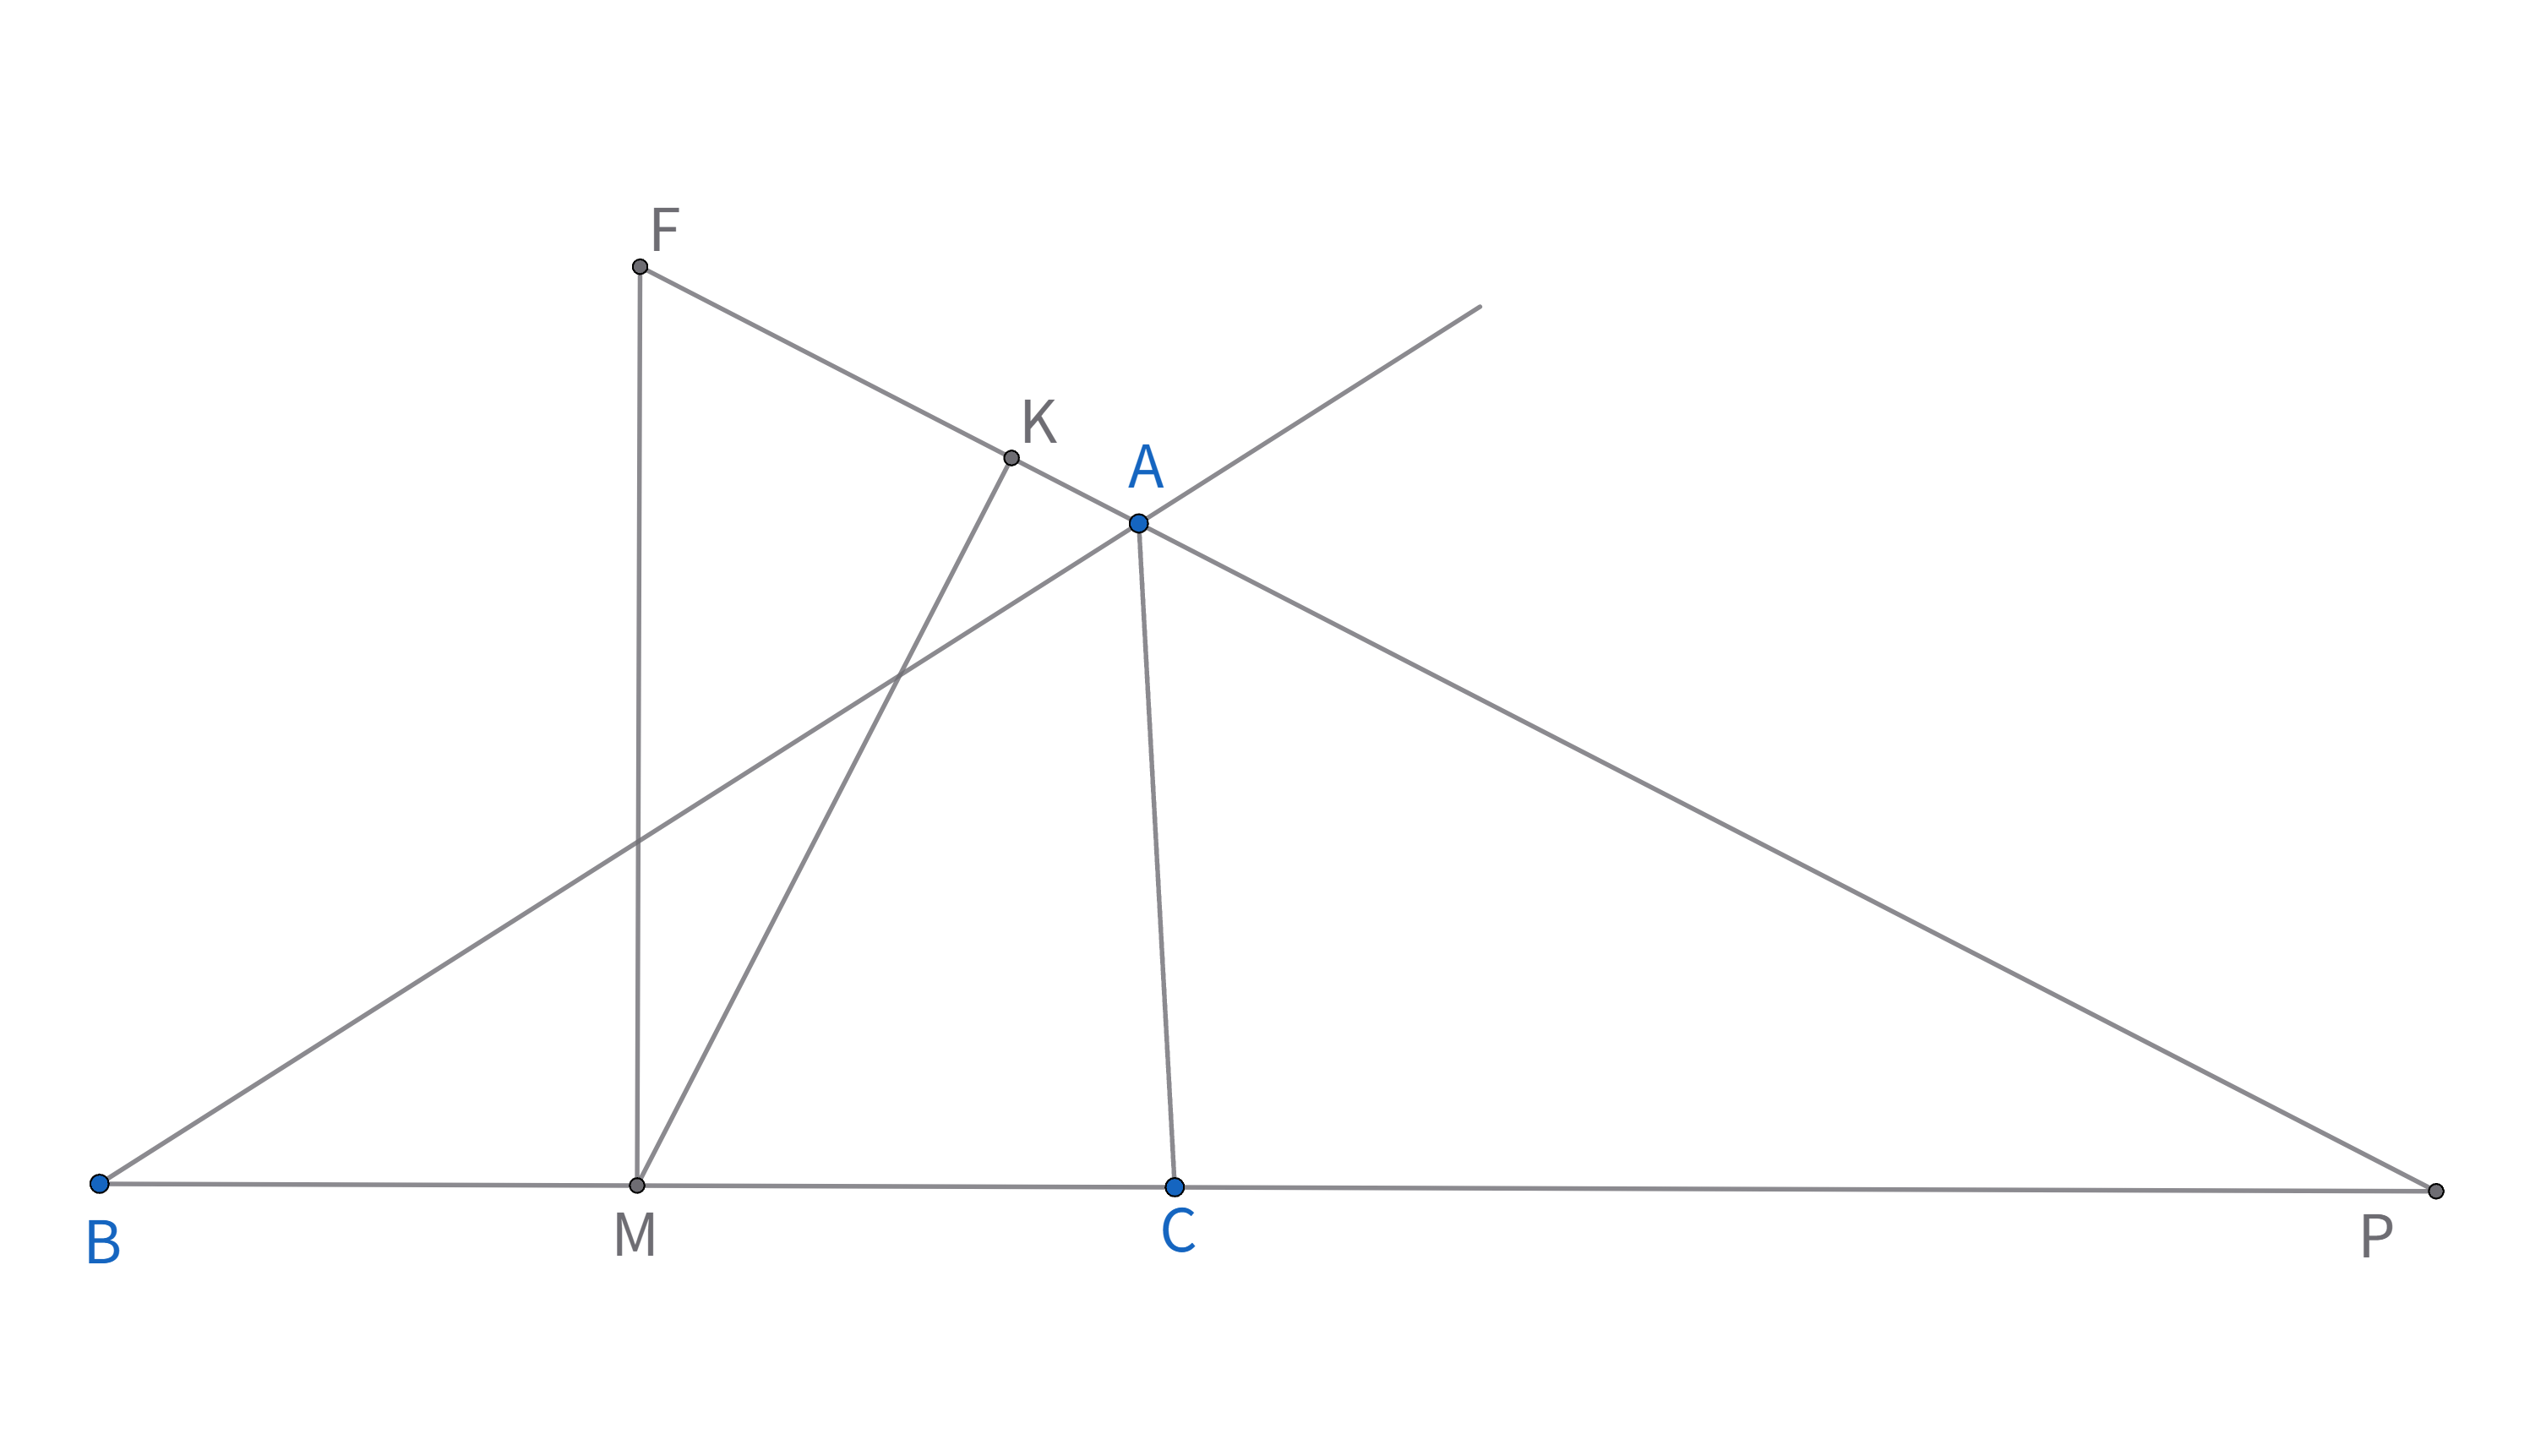
\includegraphics[width=0.8\linewidth]{figures/女子赛10年Q6.png}
\end{figure}


%-------------------------------------------------------------
\newpage
\section{2009年}
\subsection{Q2}
在 $\triangle ABC$ 中,$\angle BAC = 90^\circ$,点 $E$ 在 $\triangle ABC$ 的外接圆 $\Gamma$ 的弧 $BC$(不含点 $A$)内,$AE > EC$。连接 $EC$ 并延长至点 $F$,使得 $\angle EAC = \angle CAF$,连接 $BF$ 交圆 $\Gamma$ 于点 $D$,连接 $ED$,记 $\triangle DEF$ 的外心为 $O$。求证:$A$、$C$、$O$ 三点共线。
\begin{figure}[htbp]
	\centering
	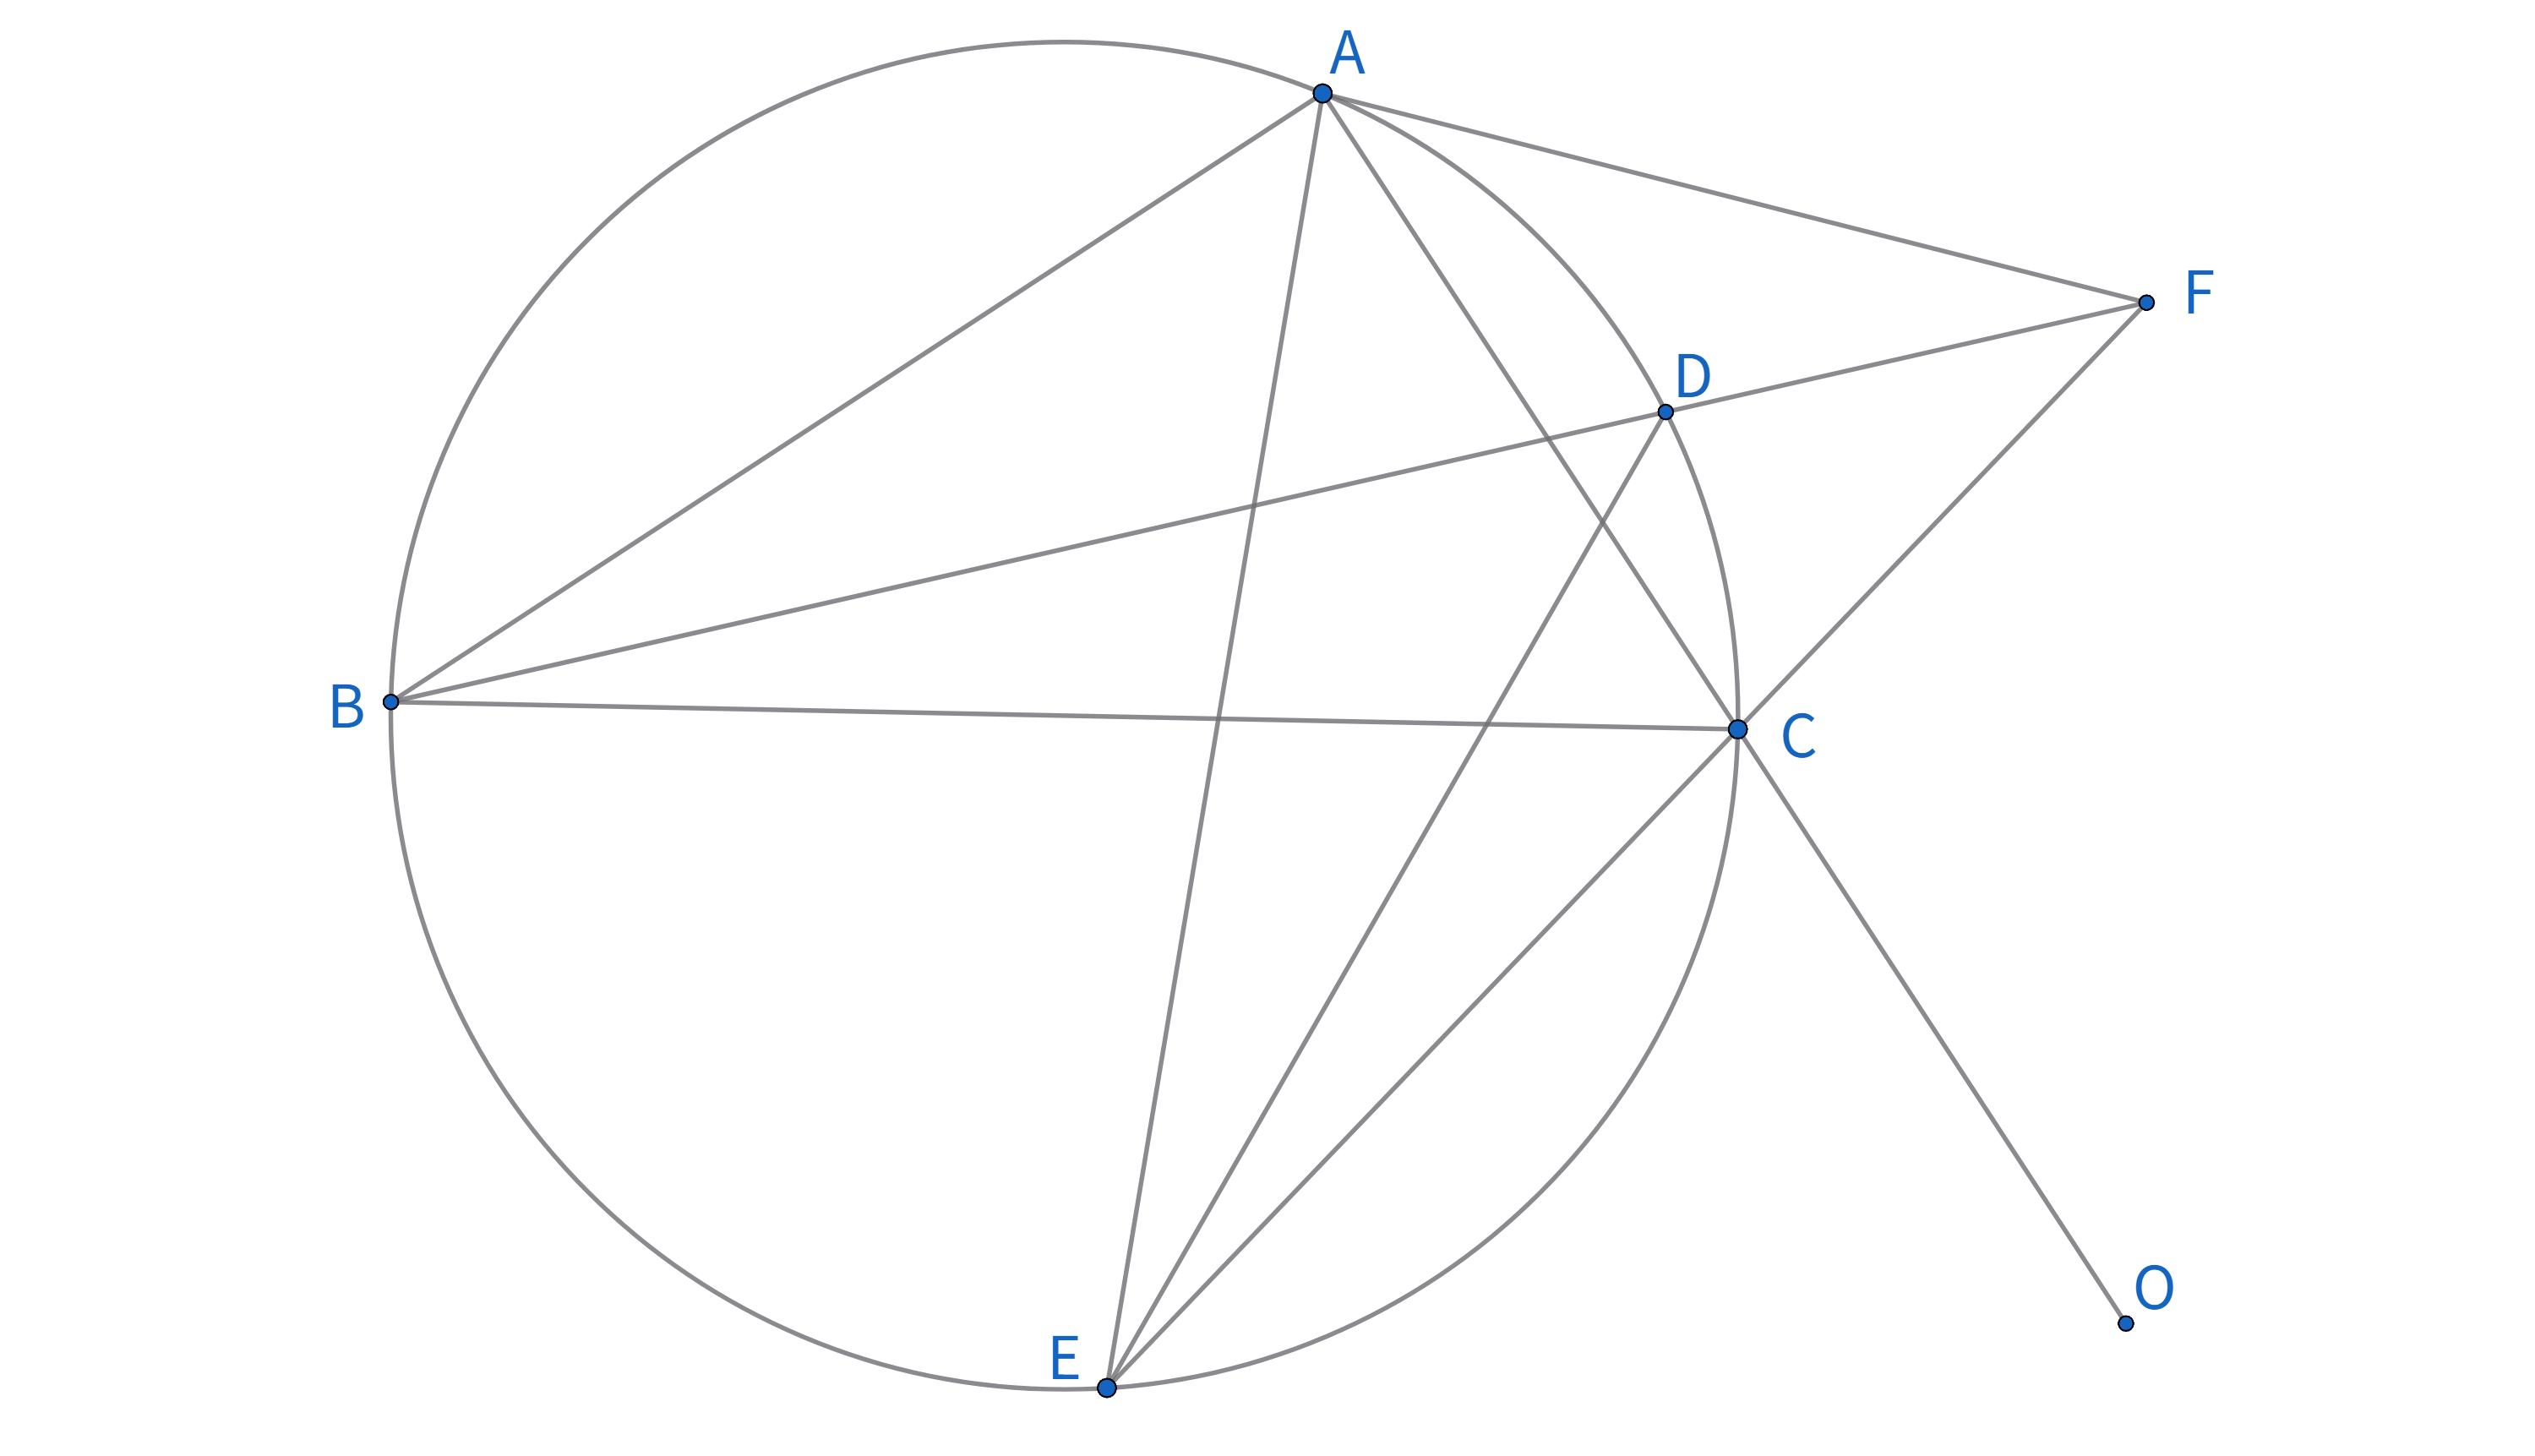
\includegraphics[width=0.8\linewidth]{figures/女子赛09年Q2.png}
\end{figure}

\subsection{Q6}
圆 $\Gamma_1$、$\Gamma_2$ 内切于点 $S$,圆 $\Gamma_2$ 的弦 $AB$ 与圆 $\Gamma_1$ 相切于点 $C$,$M$ 是弧 $AB$(不含点 $S$)的中点,过点 $M$ 作 $MN \perp AB$,垂足为 $N$。记圆 $\Gamma_1$ 的半径为 $r$,求证:$AC \cdot CB = 2r \cdot MN$。
\begin{figure}[htbp]
	\centering
	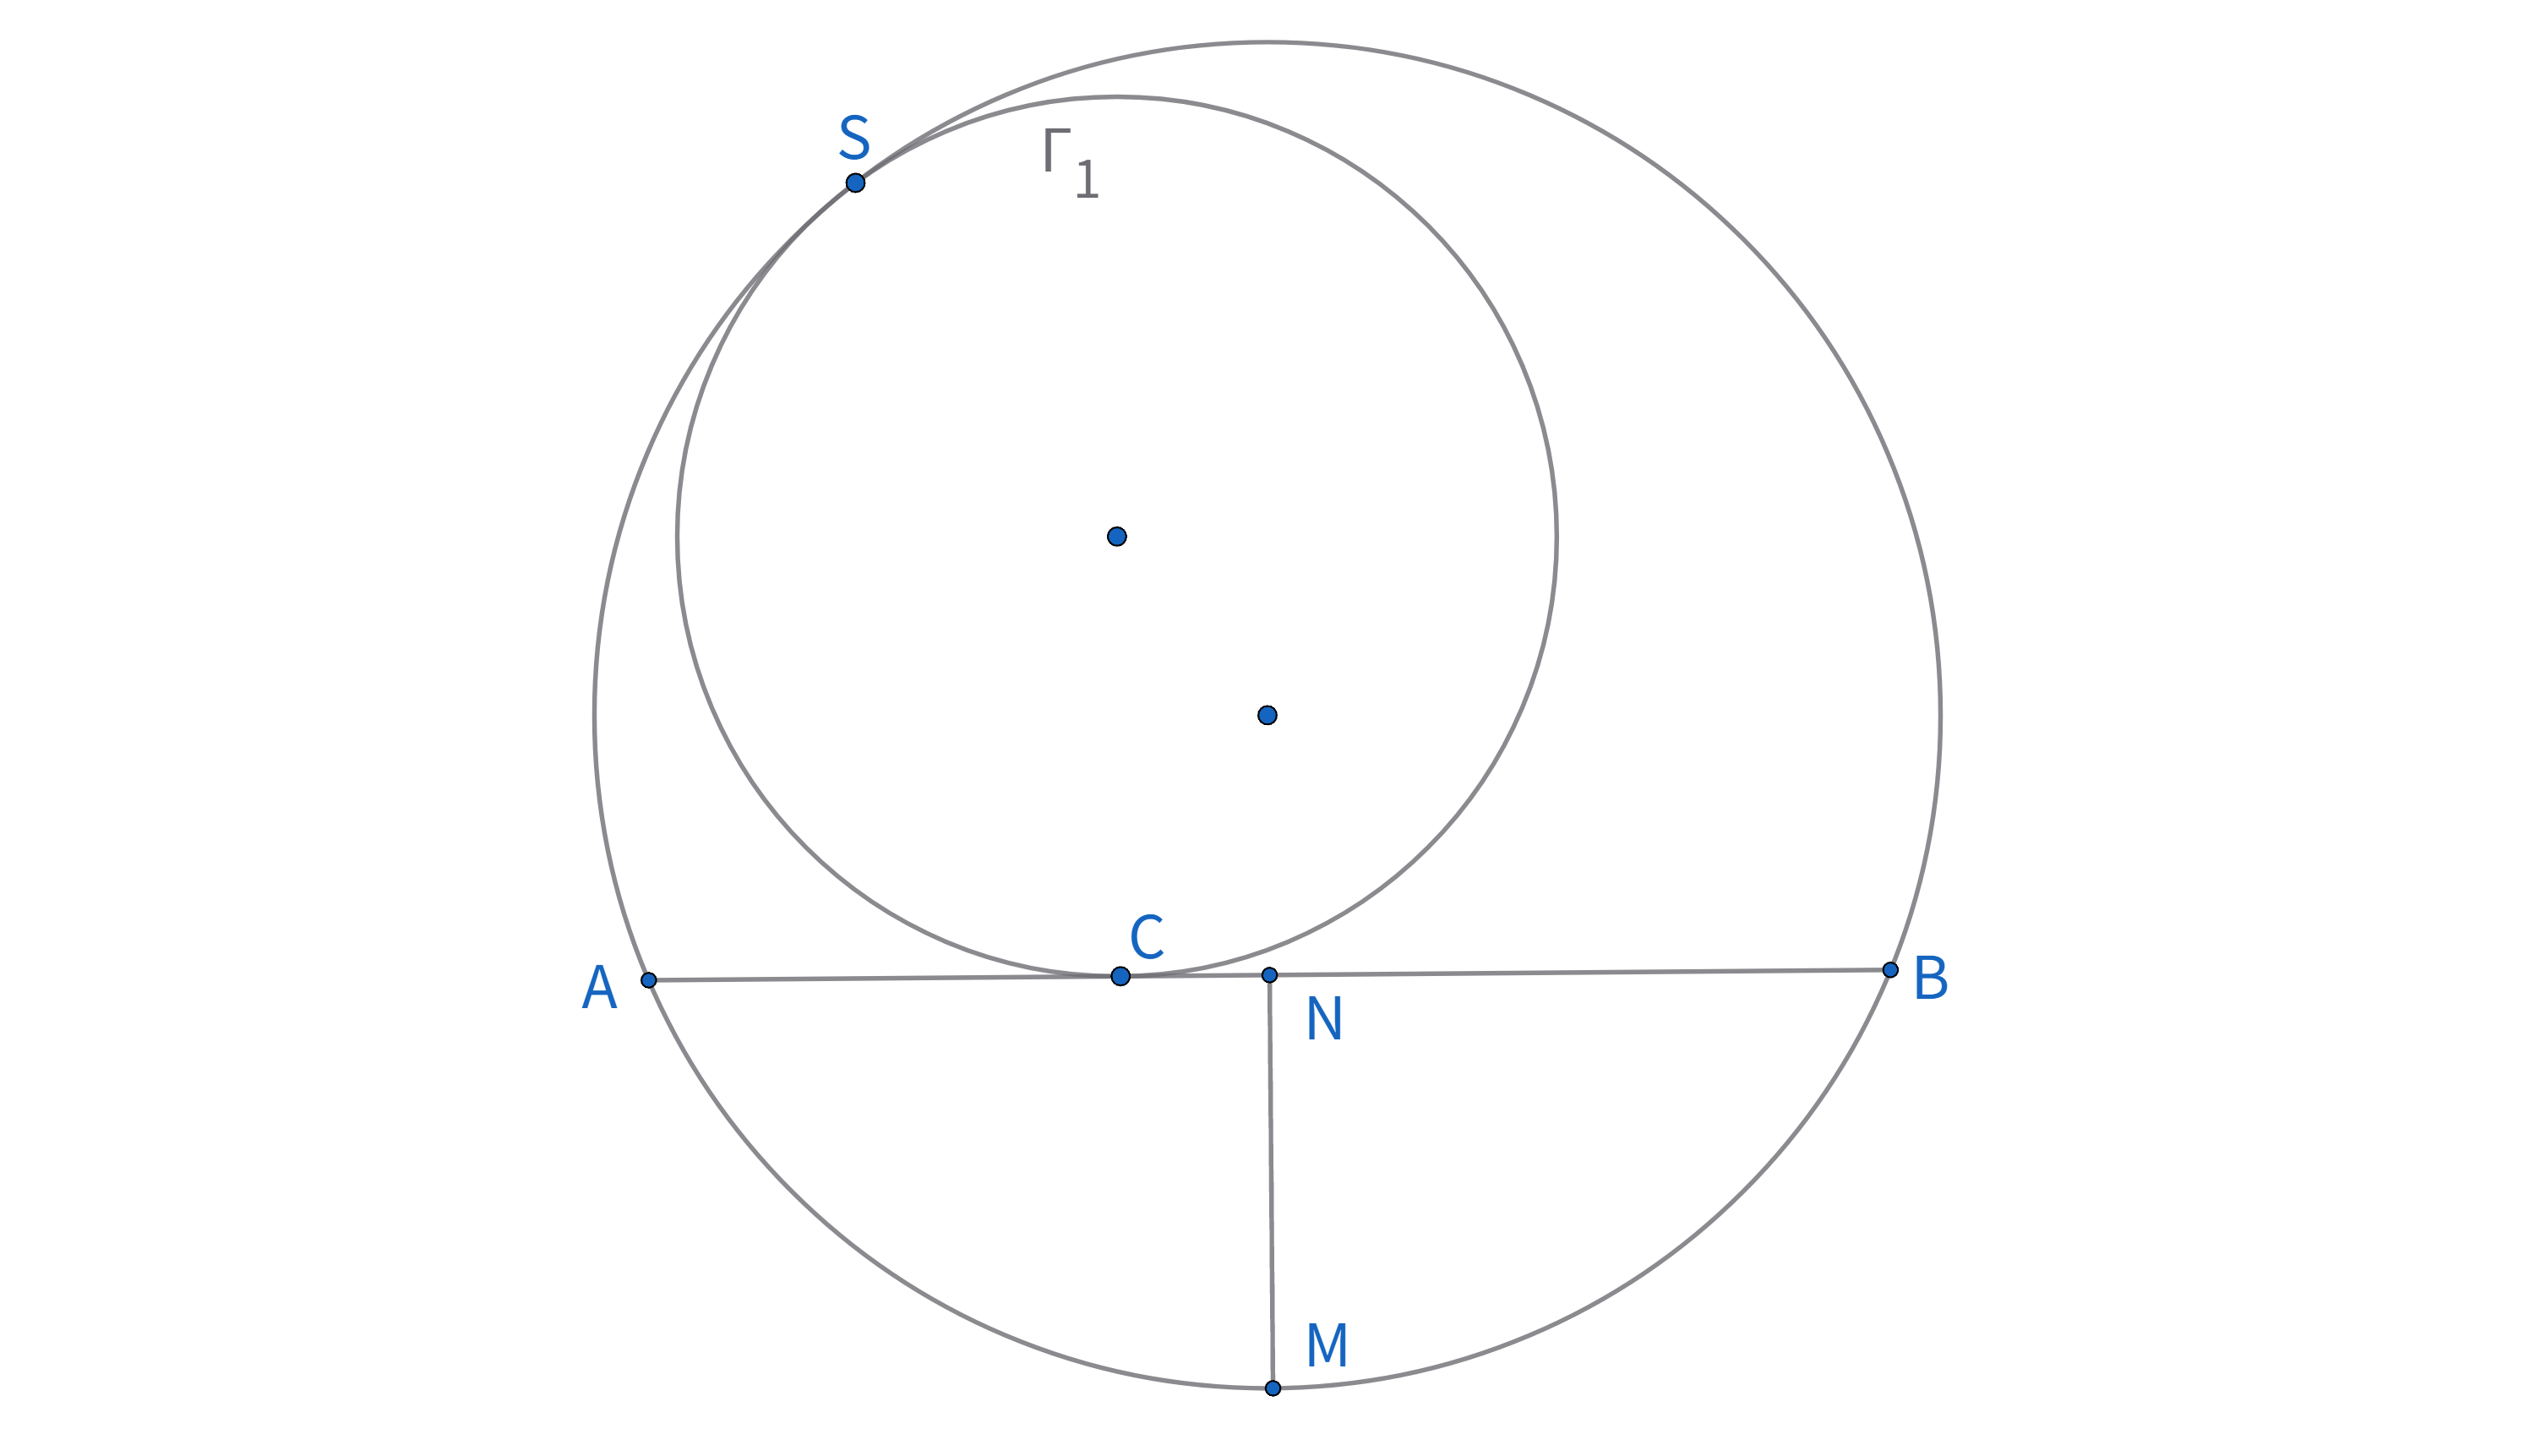
\includegraphics[width=0.8\linewidth]{figures/女子赛09年Q6.png}
\end{figure}




\end{document}